\chapter{Analysis and Results} \label{chap:results}


After analysing the dataset and implementing the optimisation algorithms, we have run several experiments to find the near-optimal points. For that, we have explored different approaches for estimating the covariance function; we have compared the different algorithm on a subset of the data;  we have run the optimisation on the full dataset; and finally, we have applied those results to a Data Assimilation Procedure. 


%%%%%%%%% COVARIANCE %%%%%%%%
\section{Covariance}

As we have seen, our approach relies heavily on a properly defined covariance estimation. We have applied several methods to find a good covariance and we are presenting them in this section. \\

From now on, we will consider that the full dataset is our pre-selected subset with $23'643$ locations. 

%\subsection{Tracer Concentration Covariance}
\subsection{Sample Covariance}

The simplest covariance estimation is the Sample (Empirical) Covariance. This Matrix is a very poor estimate, as it is singular and not positive definite and poorly conditioned. It makes it impossible to invert to use it for the GPs of our optimisation problem. \\ 

We compute the determinant of the matrix using \texttt{numpy.linalg.slogdet} for the stability of this function. It indicates us that the determinant is clearly negative, and the logarithm of the determinant's absolute value is: $-1'399'936.286$. The largest eigenvalue is: $\lambda_1 = 0.0219$ and the smallest eigenvalue is: $\lambda_p = -6.8929 \cdot 10^{-18}$.

We plot in Figure \ref{fig:cov:emp:eigs} the eigen-decomposition of this sample covariance matrix.

\begin{figure}[h!]
\centering
    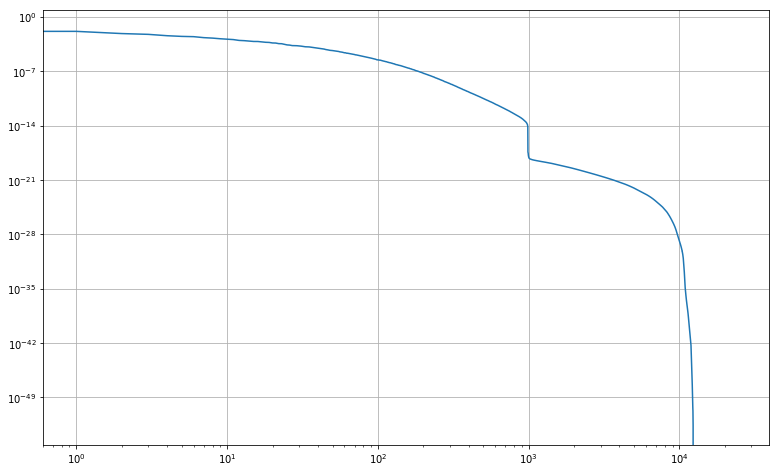
\includegraphics[width=0.7\linewidth]{figures/Covariance/Tracer_23643/cov_emp_eigenval_loglog}
    \caption{Empirical Covariance: Eigenvalues - Tracer}
    \label{fig:cov:emp:eigs}
\end{figure}

So the sample covariance matrix can not be directly used for our optimisation algorithm.  

\subsection{Shrinkage Covariance}

In this section we show the results of the class of shrinkage covariance estimators for the \textit{Tracer} Data. We use a simple \textbf{shrinkage} with shrinkage constant $\rho = 0.1$,  $\rho = 0.5$ and $\rho = 0.8$,  the \textbf{Ledoit-Wolf} Shrinkage and the \textbf{OAS} Shrinkage. 

\begin{table}[h]
\centering
    \begin{tabular}{l|ccccc}
     \toprule
        & SignDet & LogDet & $\lambda_1$ & $\lambda_p$ & $\rho$ \\ \midrule
        Empirical & ($-$) & $-1'399'936.28$ &  $0.0219$ & $-6.8929 \cdot 10^{-18}$ & -\\
        Shrinkage $\rho=0.1$ & ($+$) & $-351'807.64$ &  $0.0197$ &$3.3603\cdot 10^{-7}$ & $0.1$\\
        Shrinkage $\rho=0.5$ & ($+$) & $-314'035.58$ &  $0.0109$  &$1.6801 \cdot 10^{-6}$ & $0.5$\\
        Shrinkage $\rho=0.8$ & ($+$) & $-303'046.20$ &  $0.00438$  &$2.6882 \cdot 10^{-6}$ & $0.8$\\
        Ledoit-Wolf & ($+$) & $-406'320.19$&  $0.0217$ & $3.2867\cdot 10^{-8}$ & $0.0097811$\\
        OAS & ($+$) & $-408'903.33$ & $0.0217$ & $2.9435\cdot 10^{-8}$ & $0.0087595$ \\  \bottomrule
    \end{tabular}
    \caption{Shrinkage Comparison - Tracer}
\end{table}

\begin{figure}[h!]
\centering
    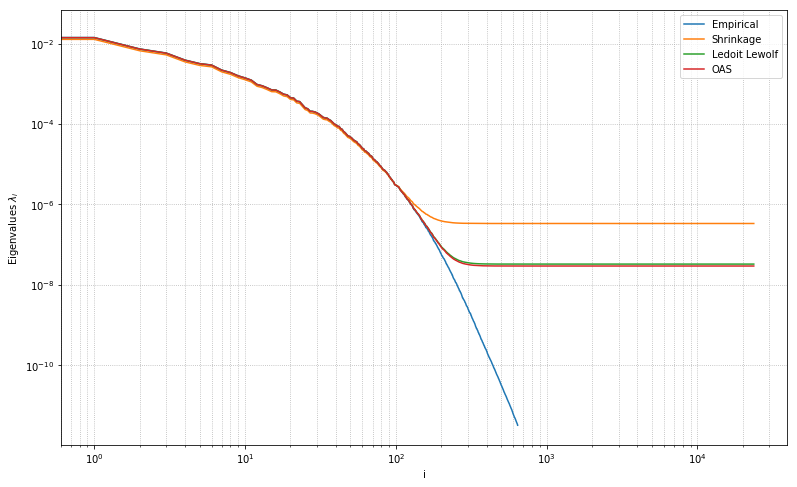
\includegraphics[width=0.8\linewidth]{figures/Covariance/Tracer_23643/cov_all_eigenval_loglog_zoom}
    \caption{Eigenvalues Covariance Comparison - Tracer}
    \label{fig:cov:comparison:eigs}
\end{figure}

As we can see the shrinkage algorithm allows to have a positive definite matrix that is very close to the original covariance matrix. It shares a lot of eigenvalues with the sample covariance matrix. This varies in function of the shrinkage constant $\rho$. For arbitrary values, $\rho = 0.1$,  $\rho= 0.5$ and  $\rho= 0.8$, we see that the smaller the shrinkage constant is, the closer we get to the sample covariance. For large constant value, we see that the upper part of the spectrum deteriorates completely, meaning that we don't have a good estimation anymore. This is perfectly logical with regards to the definition of the shrinkage which is a convex linear combination between a diagonal matrix and the sample covariance. \\

For LW and OAS, the shrinkage variable computed is close to $0.1$. The spectrums are almost identical and are resulting in very similar covariances matrixes. We see that the upper part of the spectrum is almost identical to the sample covariance matrix, but that the lower part is truncated. \\


Globally, we see that with shrinkage  the small eigenvalues get larger and that the large ones get smaller. We observe also that the determinant becomes positive, and also that it leads to a positive definite matrix. \\

As OAS gives us theoretically an optimal $\rho$ with very small error, therefore, we decide to use the \textbf{OAS estimation} of the covariance matrix for the optimisation procedure to follow.

%\subsection{Covariance on other fields}

%\subsection{Pressure Covariance}
%
%Now we study the same Covariance Estimators applied to the Pressure Field. 
%
%
%\subsubsection{Sample Covariance}
%
%Similarly, we see that the sample covariance matrix is a poor estimate of the true covariance matrix as it is not positive definite and near singular. 
%
%\begin{figure}[h!]
%\centering
%    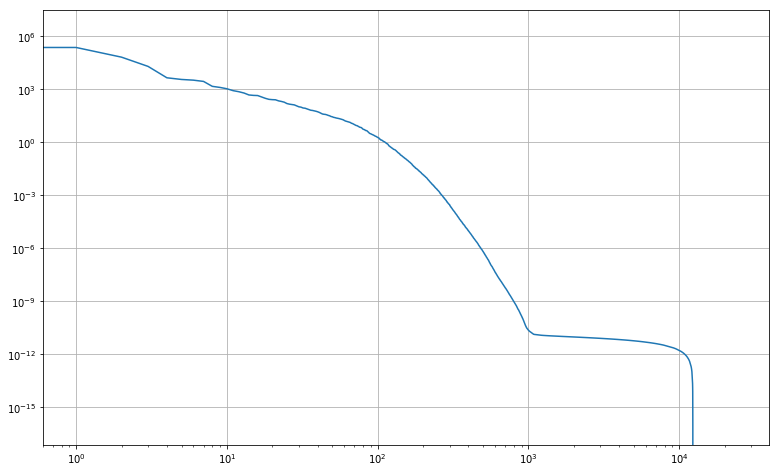
\includegraphics[width=0.8\linewidth]{figures/Covariance/Pressure_23643/cov_emp_eigenval_loglog}
%    \caption{Empirical Covariance: Eigenvalues - Pressure}
%    \label{fig:cov:emp:eigs}
%\end{figure}
%
%\subsubsection{Shrinkage Covariance}
%
%In this section we show the results of the class of shrinkage covariance estimators for the \textit{Tracer} Data. We use a simple \textbf{shrinkage} with shrinkage constant $\rho = 0.8$,  the \textbf{Ledoit-Wolf} Shrinkage and the \textbf{OAS} Shrinkage. 
%
%\begin{table}[h]
%\centering
%    \begin{tabular}{l|ccccc}
%     \toprule
%        & SignDet & LogDet & $\lambda_1$ & $\lambda_p$ & $\rho$ \\ \midrule
%        Empirical & ($-$) & $-601'246.12$ &  $2'303'868.81$ & $-8.0587 \cdot 10^{-10}$ & -\\
%        Shrinkage $\rho=0.8$ & ($+$) & $106330.01$ &  $460'863.34$  &$89.5867$ & $0.8$\\
%        Ledoit-Wolf & ($+$) & $6830.41$&  $2'276'858.60$ & $1.3129$ & $0.01172$\\
%        OAS & ($+$) & $-31'175.97$ & $2'298'501.89$ & $0.2608$ & $0.0087595$ \\  \bottomrule
%    \end{tabular}
%    \caption{Shrinkage Comparison - Pressure}
%\end{table}



%%%%%%%%% COMPARISON %%%%%%%%

\section{Comparison Optimisation Algorithms}

We have defined the three algorithms allowing for a near-optimal placement of the sensors. We have also defined an approximation of the GPs. To compare their performance and measure their limitation, we have run them on a small dataset, a subset of our main one. 
\subsection{Conditions of the Experiment}

We have defined a sphere of radius $25$m, centred close to the centre, in the middle of the propagation beam, at position $[60,35,0]$ in which are contained $3'130$ points of the mesh. By taking the intersection between those points and our selection defined in \ref{sec:preselection}, we can reduce the number of points $|S|$ to $1'295$.  The candidates are presented in Figure      \ref{fig:smallset:position}.
 \\

\begin{figure}[h!]
\centering
    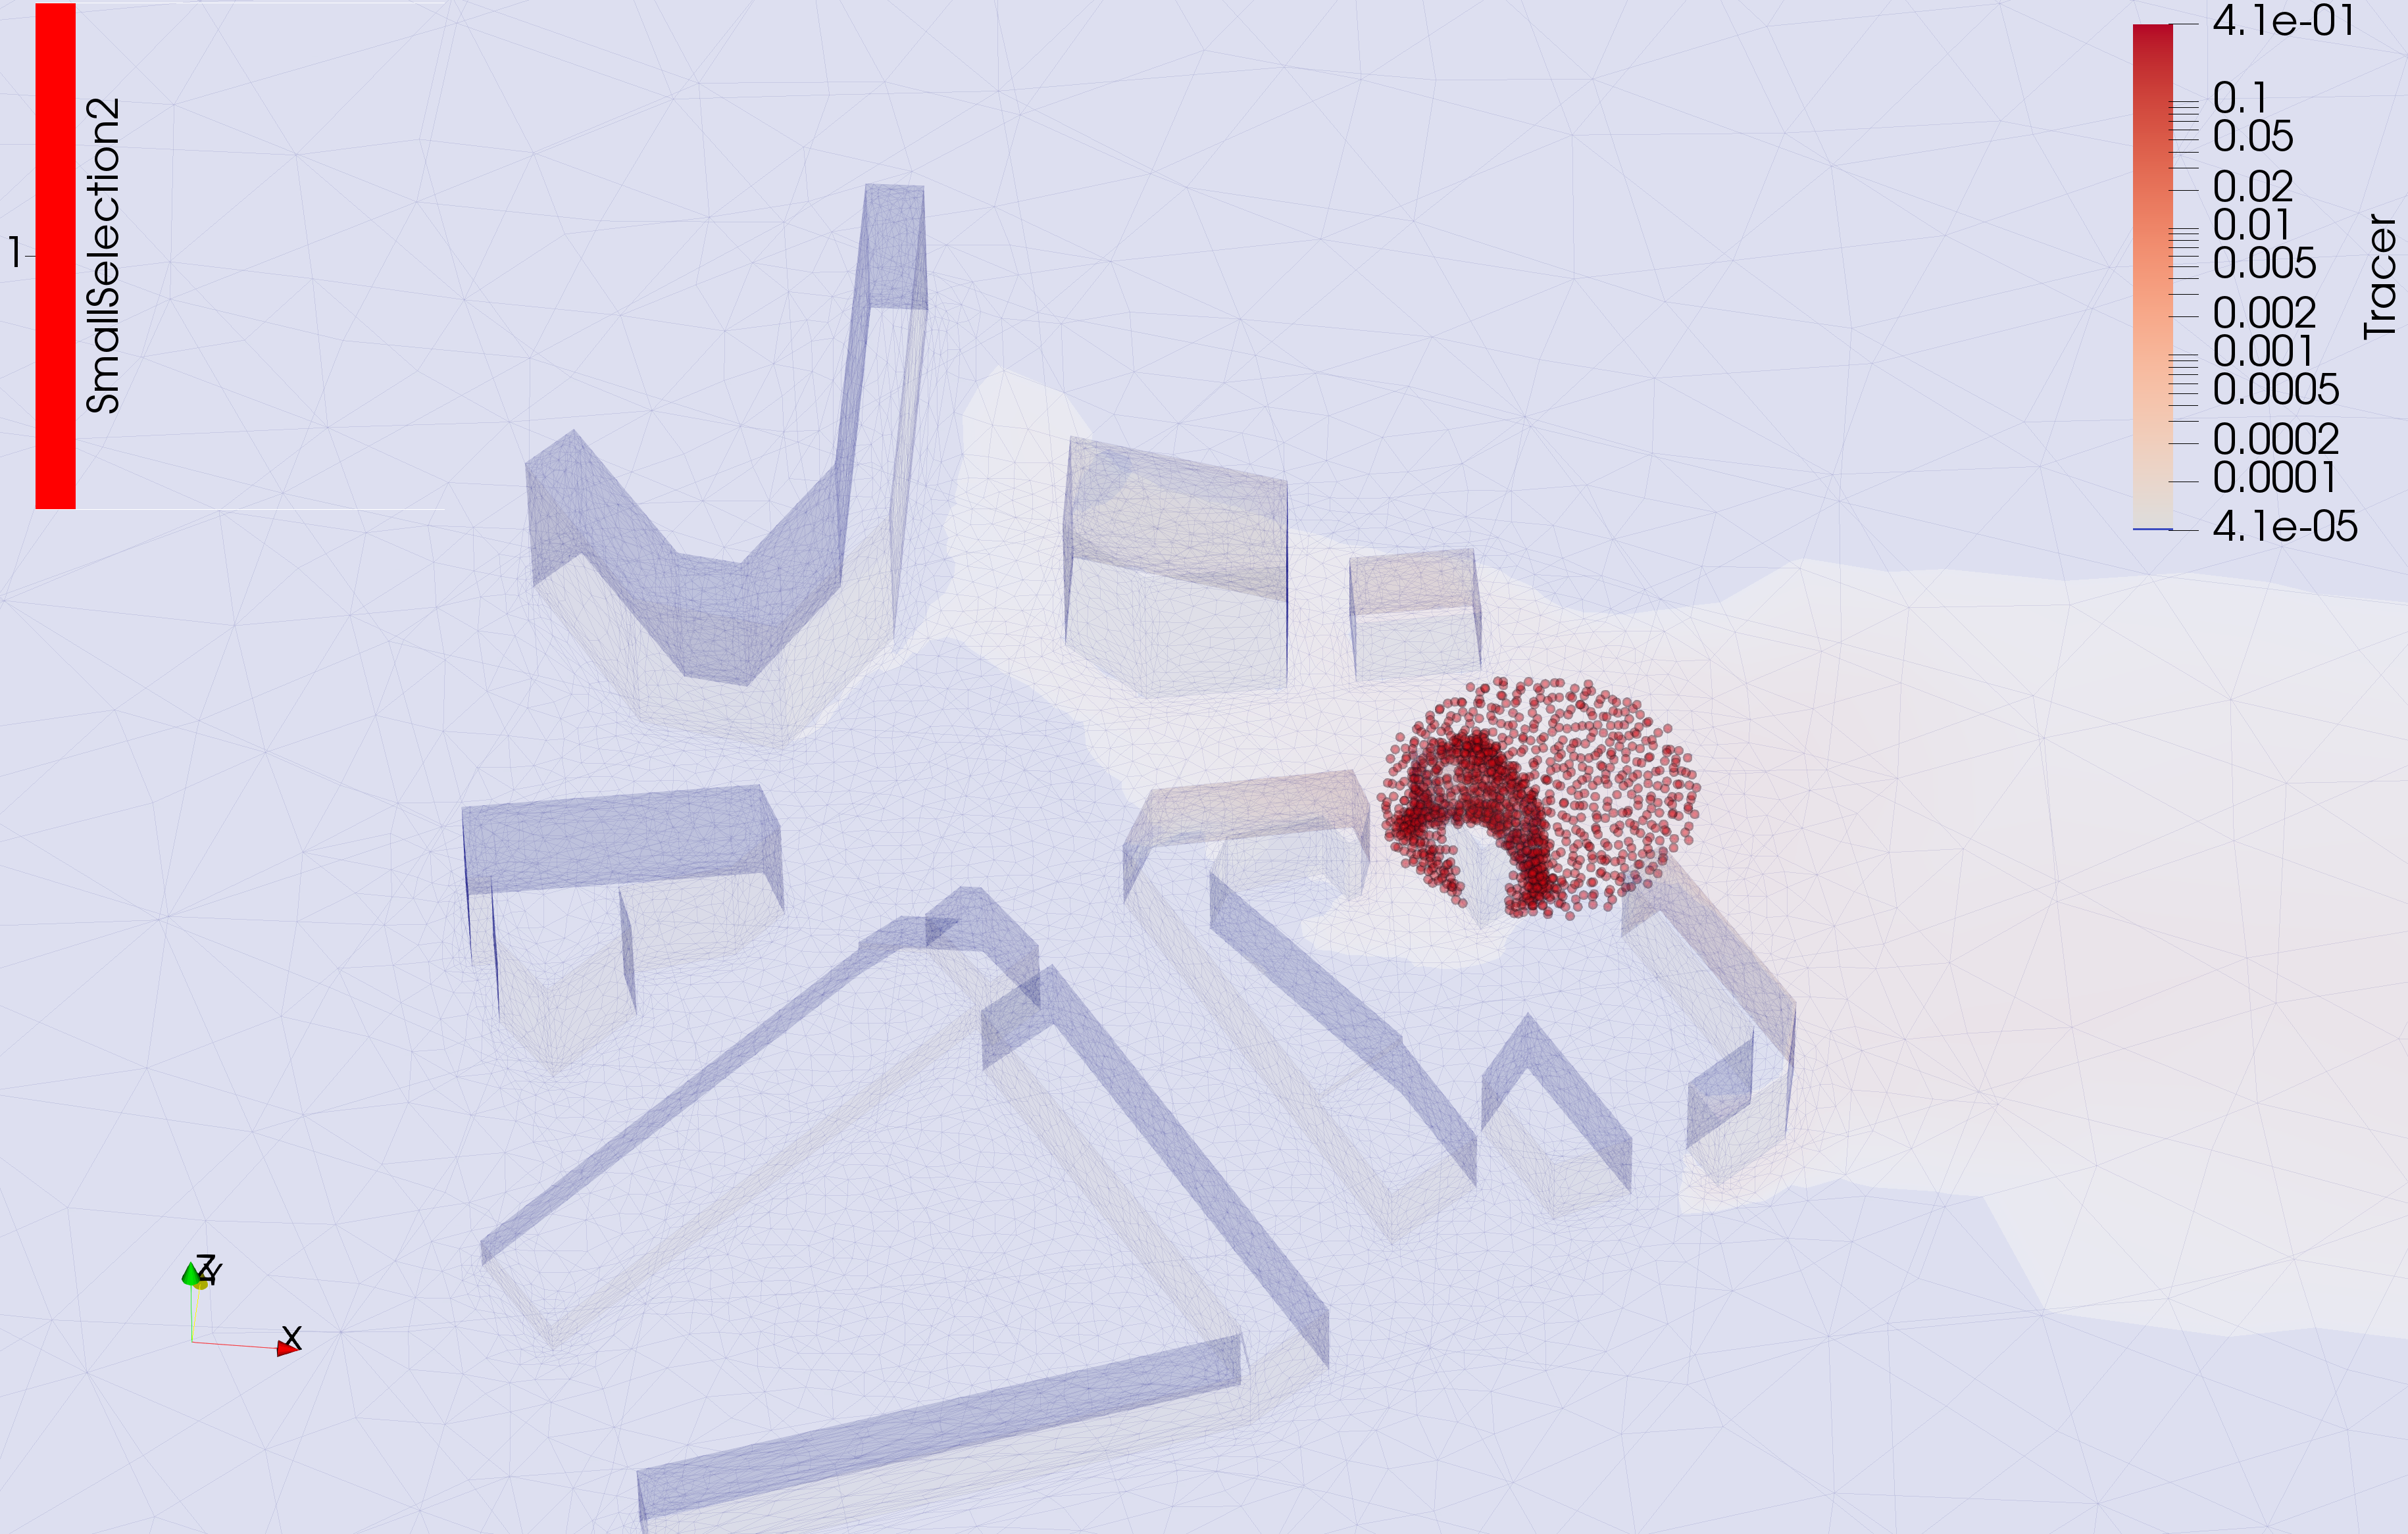
\includegraphics[width=0.8\linewidth]{figures/CompAlg/3rd/non_centered_60.35.0/candidates_screenshot}
    \caption{Small Subset Candidates}
    \label{fig:smallset:position}
\end{figure}

We compute the OAS covariance for this dataset and we will use in in the rest of the experience. The eigenvalues decomposition is shown for both the empirical covariance and the OAS estimate in Figure \ref{fig:small_cov_eig:tracer}. As shown previously we have a spectrum that is close to the original sample covariance,  only with a truncated lower part. \\

For the \textit{Tracer} we have a sample covariance that is \textbf{negative definite} with \textit{logDet} of $-39'755.06$. The OAS approximation allows us to get a \textbf{positive definite} covariance matrix with \textit{logDet} of $-19'447.95$.  \\

%For the \textit{Pressure} we have a sample covariance that is \textbf{negative definite} with \textit{logDet} of $-28'714.93$. The OAS approximation allows us to get a \textbf{positive definite} covariance matrix with \textit{logDet} of $-2'138.49$.  \\

\begin{figure}[h!]
\centering
    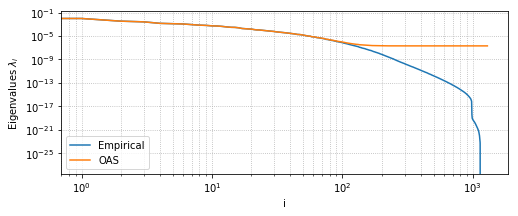
\includegraphics[width=0.7\linewidth]{figures/CompAlg/covarianceEmpOAS}
    \caption{Spectrum of Empirical and OAS covariances for Tracer}
    \label{fig:small_cov_eig:tracer}
\end{figure}

%\begin{figure}[h!]
%\centering
%    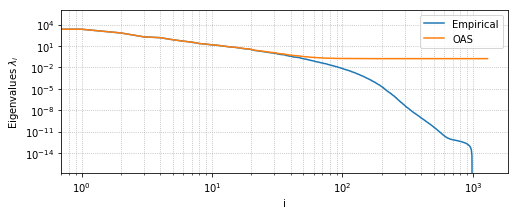
\includegraphics[width=0.7\linewidth]{figures/CompAlg/cov_emp_oas_log}
%    \caption{Spectrum of Empirical and OAS covariances for Pressure}
%    \label{fig:small_cov_eig:pressure}
%\end{figure}

Next, we are going to optimise in this space $k=10$ points with the different algorithms and compare them based on the computation time and the distance between the datasets using the NN distance defined in \ref{equ:distNN}. 

%\subsection{Optimisation on Tracer Concentration}
%In the first time, we are going to compare the performances of the different algorithms using the \textbf{Tracer Concentration} Data. 


\subsection{Greedy and Lazy Optimisation}

First, we optimise using the two first algorithms, the \textbf{greedy} and the \textbf{lazy} versions of the near-optimal sensor positioning algorithms. We will consider the output of the first algorithm as the reference for this comparison. This is because the first algorithm is the most reliable version as it covers every candidate point in its loops and relies on full GP implementation.  \\


We observe immediately that output sets given by the two methods are the same. The main difference is as expected the computation time which is much larger in the first algorithm. The Greedy Optimisation gives a result after $1043.27$s and the \textit{lazy} Optimisation gives results after $153.51 $s. The second algorithm is, for this small dataset, seven times faster than the greedy one: this is a significative difference. \\ 

The location of those points optimal points $\A^*$ is shown in green in the Figure \ref{fig:opt_small} and table \ref{tab:opt_small}. We observe that the points are well spread across space and along the wind direction. As the wind is propagating the tracer concentration, it makes sense that the sensors must be placed along this direction. \\

\begin{figure}[h!]
\centering
    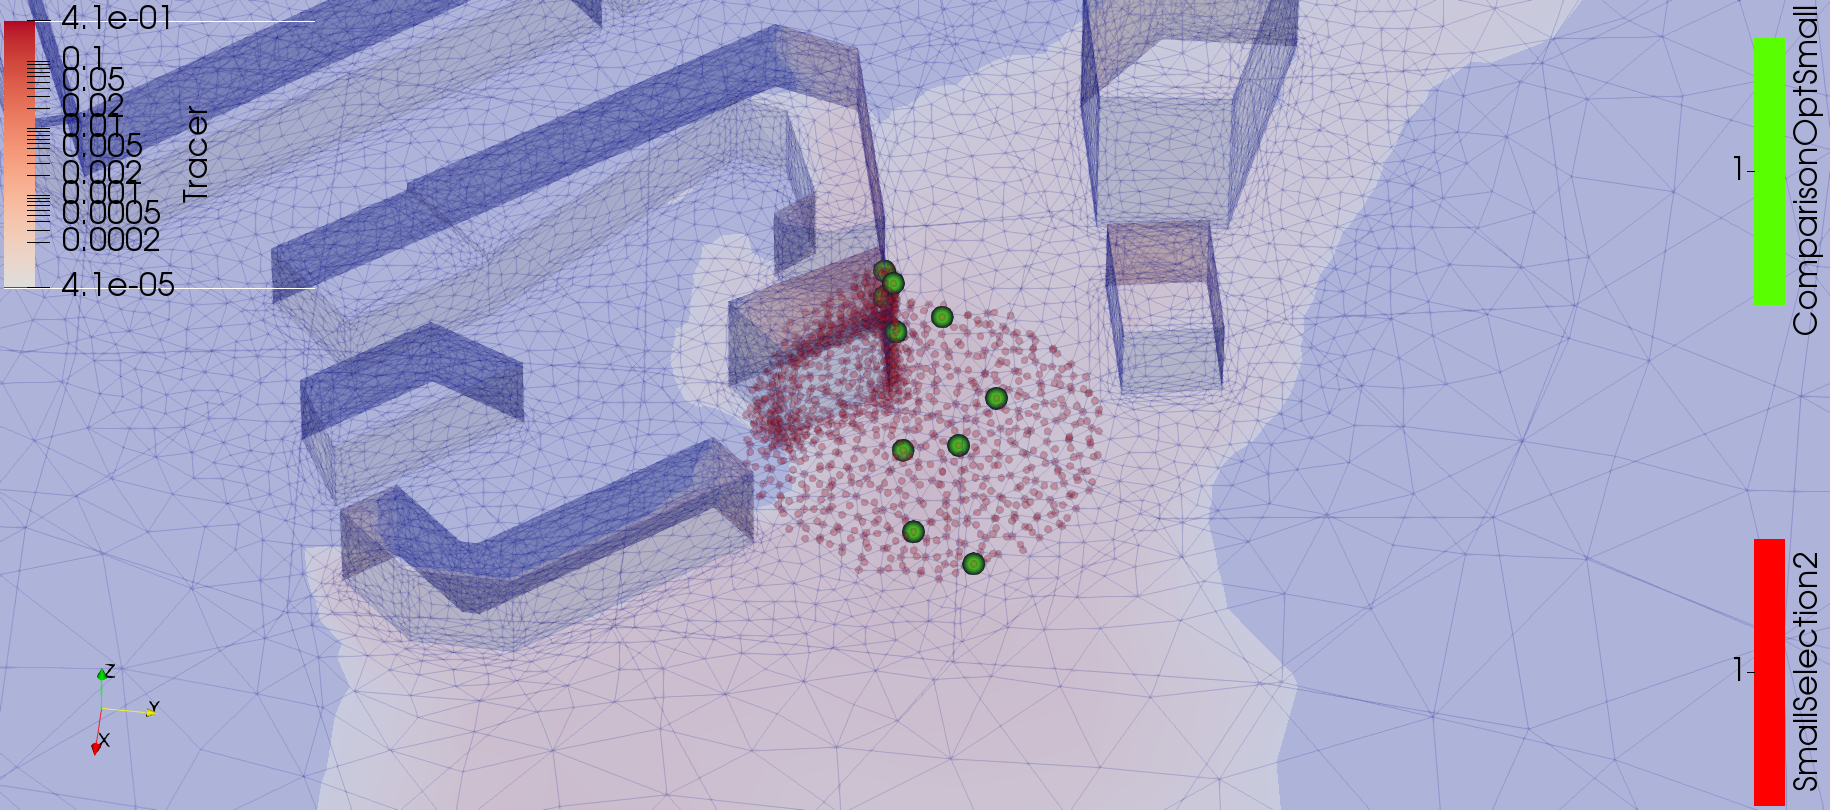
\includegraphics[width=0.8\linewidth]{figures/CompAlg/3rd/non_centered_60.35.0/optimal_screenshot}
    \caption{Optimal Points Location: Illustation}
    \label{fig:opt_small}
\end{figure}

\begin{table}[h]
\centering
\footnotesize
\begin{tabular}{l|rrrrrrrrrr}
\toprule
$\A^*$ &  52731 &  47876 &  3078  &  19782 &  26045 &  30511 &  26754 &  81507 &  11608 &  3903  \\
\midrule
X &  61.31 &  43.55 &  77.31 &  38.75 &  48.23 &  50.48 &  52.36 &  43.10 &  82.40 &  62.01 \\
Y &  40.06 &  27.62 &  35.55 &  35.26 &  29.38 &  30.04 &  44.37 &  27.52 &  44.48 &  32.39 \\
Z &   1.52 &  16.40 &   1.45 &   1.80 &  19.53 &  11.79 &   1.62 &  10.23 &   1.96 &   0.20 \\
\bottomrule
\end{tabular}
\caption{Optimal Points Locations }
\label{tab:opt_small}
\end{table}


We also can plot the Mutual Information Gain $\delta_{y^*}$at each sensor placement on Figure \ref{fig:compAlg:MIGAIN}. What we can see confirms that our Mutual Information is sub-modular, as the Mutual Information Gain is monotonically decreasing. 


\begin{figure}[h!]
\centering
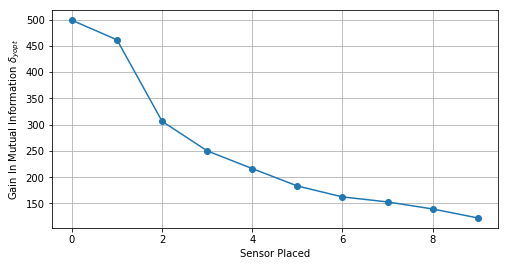
\includegraphics[width=0.6\linewidth]{figures/CompAlg/3rd/non_centered_60.35.0/MIGain}
\caption{Mutual Information Gain for each sensor - Greedy \& Lazy Algorithms}
\label{fig:compAlg:MIGAIN}
\end{figure}


\subsection{Local Kernels Optimisation}

The 3rd Algorithm that we are going to use is the one that is scalable to larger datasets. This scalability is dependent on the parameter $\epsilon$, the thresholding parameter of the covariance. As a consequence the number of selected covariates  $|N(y_{opt},\epsilon)| \leq d $ is fluctuating and influences greatly the speed of the algorithm. It is directly linked to the GP and the size of the covariance matrix to invert.  \\ 

This is why the threshold $\epsilon$ has to be chosen carefully. We are going to show that the speed, the NN distance and the parameter d varies according to $\epsilon$, before choosing a value that will be used for the full-scale optimisation. We compute of a range of values for $\epsilon$ all those results and show them in table \ref{tab:comp:results} and in Figure \ref{fig:comp:results}. \\



\begin{table}[h]
\centering
\scriptsize
\begin{tabular}{l|cccccccccc}
  \toprule
  Threshold $\epsilon$ & $10^{-10} $ &  $10^{-9}$ & $10^{-8}$ & $10^{-7}$ & $10^{-6}$ & $10^{-5}$ & $10^{-4}$ & $10^{-3}$ & $10^{-2}$ & $10^{-1}$ \\
    \midrule
  Distance [m]       &    0.00 &    0.00 &    0.00 &    0.00 &   1.248 &  2.783 & 4.693 & 11.058 & 11.058 & 11.058 \\
Time [s]       & 1660.85 & 1617.92 & 1500.63 & 1151.68 &  520.36 &  60.88 &  2.44 &   1.74 &   3.25 &   2.13 \\
Average d & 1289.40 & 1288.20 & 1284.80 & 1245.60 & 1029.60 & 510.50 & 15.20 &   0.00 &   0.00 &   0.00 \\
  \bottomrule
\end{tabular}
\caption{Local Kernel Results - Tracer}
\label{tab:comp:results}
\end{table}

\begin{figure}[h]
\centering
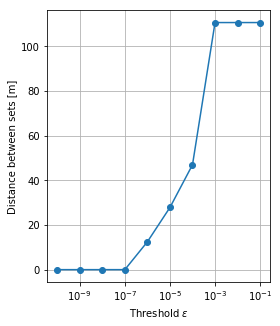
\includegraphics[height=0.33\linewidth]{figures/CompAlg/3rd/non_centered_60.35.0/comp_dist}
~
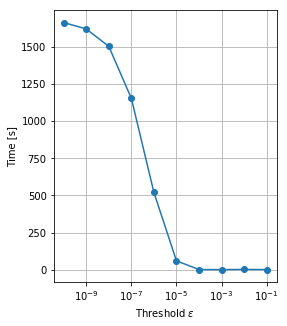
\includegraphics[height=0.33\linewidth]{figures/CompAlg/3rd/non_centered_60.35.0/comp_Time}
~
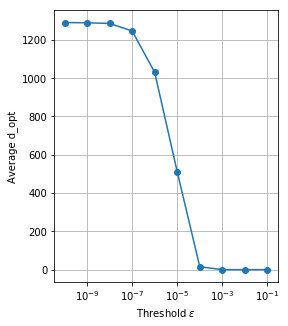
\includegraphics[height=0.33\linewidth]{figures/CompAlg/3rd/non_centered_60.35.0/comp_d_opt}
\caption{Local Kernels: Distance, Time and d, in function of $\epsilon$ - Tracer}
\label{fig:comp:results}
\end{figure}

We see that computation time is correlated with the average number of correlates d. For a threshold bellow $10^{-7}$, we see that the algorithm selects almost every point available and therefore we have computation times of the order of the greedy algorithm. The optimised set of points is then also the same as the greedy and lazy algorithms.\\

By increasing the threshold, we find that the computation time and the number of covariates decrease at the expense of the accuracy represented by the increase in the NN distance between this dataset and the optimal one. We observe also that for $\epsilon > 10^{-3}$, the number of covariates selected d is equal to zero which means that the algorithm updates every position at each iteration and uses for the optimisation only the values of the original covariance, without conditioning them, as the observed set is empty.  \\

Therefore we need to \textbf{fix the threshold} at around $ \epsilon_{opt} = 10^{-6}$, so that the error is still small and the computation time substantially reduced. This threshold will be used on the full-scale optimisation of Tracer Concentration Data.  \\ 


By relocating the centre of the selection sphere, we observe that the optimal threshold is very different from one zone to the other. For example, if we place the subset in a zone where the tracer data is almost always null, we see that the threshold needs to be much smaller to get any results. This is why the value we have chosen was optimised for an area where there is some relevant data. 


\subsection{Approximated Gaussian Processes}

Alternatively, we use the approximation method developed earlier relying on the TSVD of the data, applied to algorithm 2. We proceed to the optimisation of the dataset using different values for the truncation parameter $\tau$. We then plot the computation time and the set distance to the results of the greedy algorithm in function of the truncation parameter in Figure \ref{fig:small_set:tsvd}. \\

\begin{figure}[h]
\centering
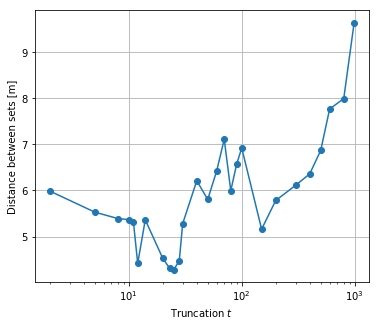
\includegraphics[height=0.33\linewidth]{figures/CompAlg/tsvd/dist_trunc}
~
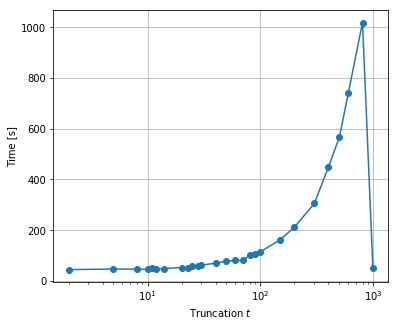
\includegraphics[height=0.33\linewidth]{figures/CompAlg/tsvd/time_trunc}
\caption{TSVD Approximation: Distance and Time in function of $\tau$}
\label{fig:small_set:tsvd}
\end{figure}

As we can see the computation time increases exponentially with $\tau$ and it is then reduced when $\tau$ gets larger than $n=988$.  For the NN distance between those sets and the optimal sets of algorithm 1, we see that it is quite low at the for a small $\tau$, and it reaches a minimum at $\tau_{opt} = 25$. For larger values, the distance is strongly increasing.  We will keep this method and the optimal truncation parameter, for testing on the full dataset in the following section. \\

It is important to mention that the result is here empirical, and that some methods providing optimal parameters are given by \citet{arcucci_optimal_2019}. In this publication, the dataset used is similar and the optimal truncation found is of the same order.  \\

%\subsection{Optimisation on Pressure}
%
%
%
%Now, we are going to compare the performances of the different algorithms using the \textbf{Pressure} Data. 
%
%\subsubsection{Greedy and Lazy Optimisation}
%
%Similarly to the case of \textbf{Tracer}, we consider that the optimal results for this configuration are given by the greedy and lazy algorithms. \\
%
%The optimal set is given in table \ref{tab:opt_small:pressure} and illustrated on Figure \ref{fig:opt_small:pressure}. The points are here too well spread on the optimisation space. They are even situated often near the border of the space. 
%
%
%\begin{figure}[h!]
%\centering
%    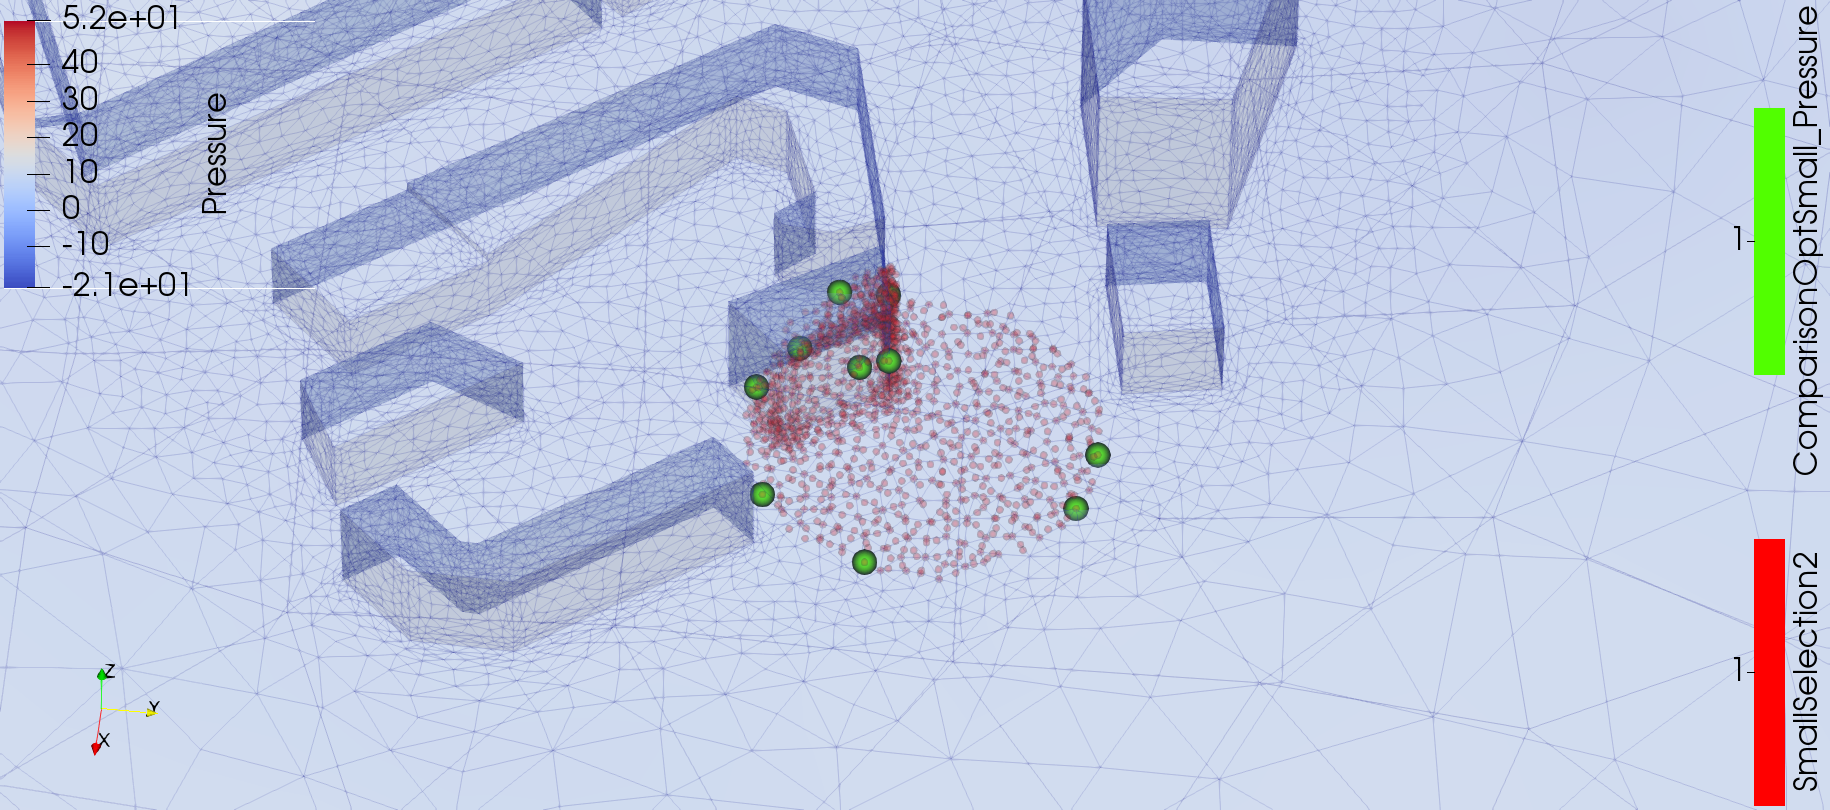
\includegraphics[width=0.8\linewidth]{figures/CompAlg/3rd/pressure_non_centered/optimal_screenshot}
%    \caption{Optimal Points Location: Illustation - Pressure}
%    \label{fig:opt_small:pressure}
%\end{figure}
%
%\begin{table}[h]
%\centering
%\footnotesize
%\begin{tabular}{l|rrrrrrrrrr}
%\toprule
%$\A^*$ &  17899 &  71227 &  71952 &  96870 &  78155 &  28083 &  40511 &  9050  &  74654 &  4146  \\
%\midrule
%X &  47.48 &  54.57 &  49.85 &  73.15 &  40.16 &  57.36 &  69.55 &  83.24 &  52.45 &  60.24 \\
%Y &  16.26 &  25.44 &  22.08 &  14.06 &  27.83 &  11.37 &  57.31 &  29.43 &  29.29 &  59.37 \\
%Z &   2.77 &   8.37 &  18.50 &   1.47 &   7.22 &   5.44 &   0.20 &   1.19 &   7.74 &   0.89 \\
%\bottomrule
%\end{tabular}
%\caption{Optimal Points Locations - Pressure}
%\label{tab:opt_small:pressure}
%\end{table}
%
%\subsubsection{Local Kernels Optimisation}
%
%We also apply the local kernel method to the Pressure Data, and we obtain the results presented in table \ref{tab:comp:results:pressure} and Figure \ref{fig:comp:results:pressure}. The threshold $\epsilon$ varies here between $60$ and $90$, as the threshold value is dependant of the data. \\
%
%We get the same kind of behaviour than in the case of the \textit{Tracer} Data. We choose the optimal threshold $\epsilon^* = 72$. For this value we have a good balance between accuracy and computation time. 
%
%
%
%\begin{table}[h]
%\centering
%\scriptsize
%\begin{tabular}{l|rrrrrrrrrr}
%\toprule
%Threshold $\epsilon$ &     60  &     65  &     70  &    75  &    80  &    82  &    84  &    86  &    88  &    90     \\
%\midrule
%Distance [m]       &    0.00 &    6.62 &   62.98 &  83.54 &  90.57 & 103.48 & 121.92 & 134.86 & 125.57 & 124.73   \\
%Time [s]        & 1217.57 & 1136.29 &  858.54 & 199.86 &  81.43 &  30.06 &  15.18 &   7.95 &   5.47 &   3.89   \\
%Average d & 1289.50 & 1287.30 & 1060.50 & 281.10 & 376.70 & 240.50 & 170.10 &  96.60 &  69.90 &  33.50   \\
%\bottomrule
%\end{tabular}
%\caption{Local Kernel Results - Pressure}
%\label{tab:comp:results:pressure}
%\end{table}
%
%\begin{figure}[h]
%\centering
%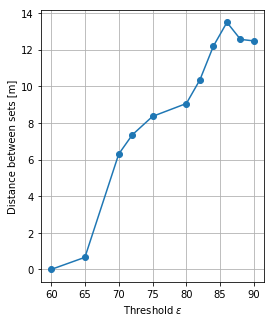
\includegraphics[height=0.33\linewidth]{figures/CompAlg/3rd/pressure_non_centered/comp_dist}
%~
%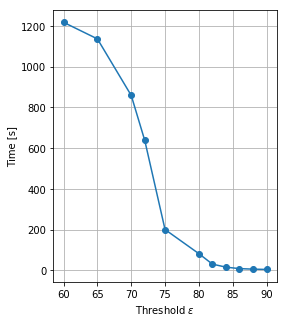
\includegraphics[height=0.33\linewidth]{figures/CompAlg/3rd/pressure_non_centered/comp_Time}
%~
%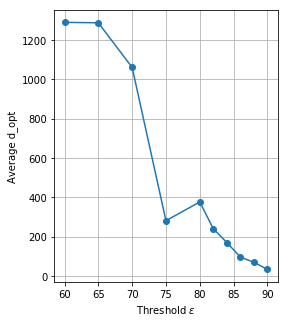
\includegraphics[height=0.33\linewidth]{figures/CompAlg/3rd/pressure_non_centered/comp_d_opt}
%\caption{Local Kernels: Distance, Time and d, in function of $\epsilon$ - Pressure}
%\label{fig:comp:results:pressure}
%\end{figure}
%
%
%
%
%
%\subsubsection{Approximated Gaussian Processes}
%
%Here we apply also the method based on TSVD, which reduces the dimension of the data to compute an approximate GP. In the Figure \ref{fig:small_set:tsvd:pressure}, we plot in function of the truncation parameter the the distance between the set and the optimal set found by algorithm 1.
%
%
%
%\begin{figure}[h]
%\centering
%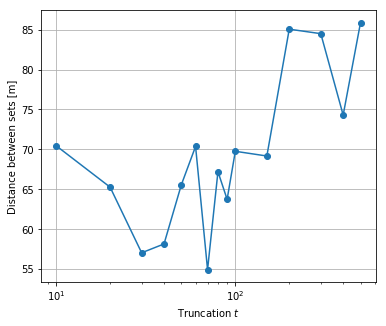
\includegraphics[height=0.33\linewidth]{figures/CompAlg/tsvd/dist_trunc_pressure}
%~
%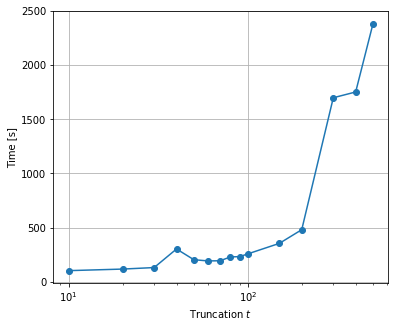
\includegraphics[height=0.33\linewidth]{figures/CompAlg/tsvd/time_trunc_pressure}
%\caption{TSVD Approximation: Distance and Time in function of $\tau$ - Pressure}
%\label{fig:small_set:tsvd:pressure}
%\end{figure}
%
%We have similar results compared to the \textit{Tracer} field. We choose a truncation parameter $\tau=25$, which has a good balance between computation time and accuracy. 

%%%%%%%%% OPTIMISATION %%%%%%%%

\section{Full Scale Optimisation Results}

After the analysis of different algorithm results on a smaller dataset, we are now going to use the most scalable algorithms with the appropriate parameters on the full dataset. The set of points used is the preselected dataset containing $23'643$ locations. \\

In this section, we will present the results of two optimisations, compare them in term of computation speed and proximity. 


%\subsection{Optimisation on Tracer Concentration}


\subsection{Local Kernel Algorithm} \label{sec:res:localK}

We first use the Local Kernel Algorithm \ref{alg:local}. The covariance between the points is computed using the OAS estimator. \\


For this experiment we used the previously defined value of threshold: $\epsilon = 10^{-6}$. Such that the number of points highly correlated to the last positioned sensor is $|N(y_{opt},\epsilon)| \leq d $. \\ 

The algorithm computes the following results in $23797.2$ seconds or $6.61$ hours. \\

We are computing for each iteration the size of this set. This number is directly linked to the size of the covariance matrix being inverted in the GPs. As we are placing 10 sensors, we have 10 values of this quantity that is computed at each iteration of the main loop. Results can be found in table \ref{tab:full:d_opt}. The average value is $4'374.7$. This shows that indeed the optimisation problem is solved in a reduced time as it doesn't use all the $23'643$ locations of our dataset, but $18.50$\% of it.   \\

\begin{table}[h]
    \centering
    \begin{tabular}{l|cccccccccc}
    \toprule
    Sensor & 1 & 2 & 3 & 4 & 5 & 6 & 7 & 8 & 9 & 10 \\     \midrule
        $|N(y_{opt},\epsilon)|$ & 4338 & 4938 & 5066 & 5362 & 4239 & 4164 & 3377 & 4632 & 3511 & 4120 \\     \bottomrule

    \end{tabular}
    \caption{Number of highly correlated points at each iteration}
    \label{tab:full:d_opt}
\end{table}


We visualise the position of the optimal set of sensor points $\A^*$ at different scales in Figure \ref{fig:full_set:position:zoom}. The coordinates of the points are expressed in the table \ref{tab:full:data}. \\


\begin{table}[h]
\centering
\footnotesize
\begin{tabular}{l|rrrrrrrrrr}
\toprule
$\A^*$ &  56588 &  52731 &  73959 &  43278 &  3078  &  19782 &  56257 &  55640 &  10357 &  54786 \\ \midrule
X &  41.61 &  61.31 &  30.32 &  22.79 &  77.31 &  38.75 &  91.19 &  50.10 &  62.13 &   1.62 \\
Y &  27.21 &  40.06 &  26.06 &  25.81 &  35.55 &  35.26 &  35.16 &  29.00 &  45.23 &  19.99 \\
Z &  16.73 &   1.52 &  11.19 &  11.79 &   1.45 &   1.80 &   1.82 &  16.41 &   1.64 &  13.81 \\
\bottomrule
\end{tabular}
\caption{Optimal Points Locations - Tracer}
\label{tab:full:data}
\end{table}



\begin{figure}[h!]
\centering
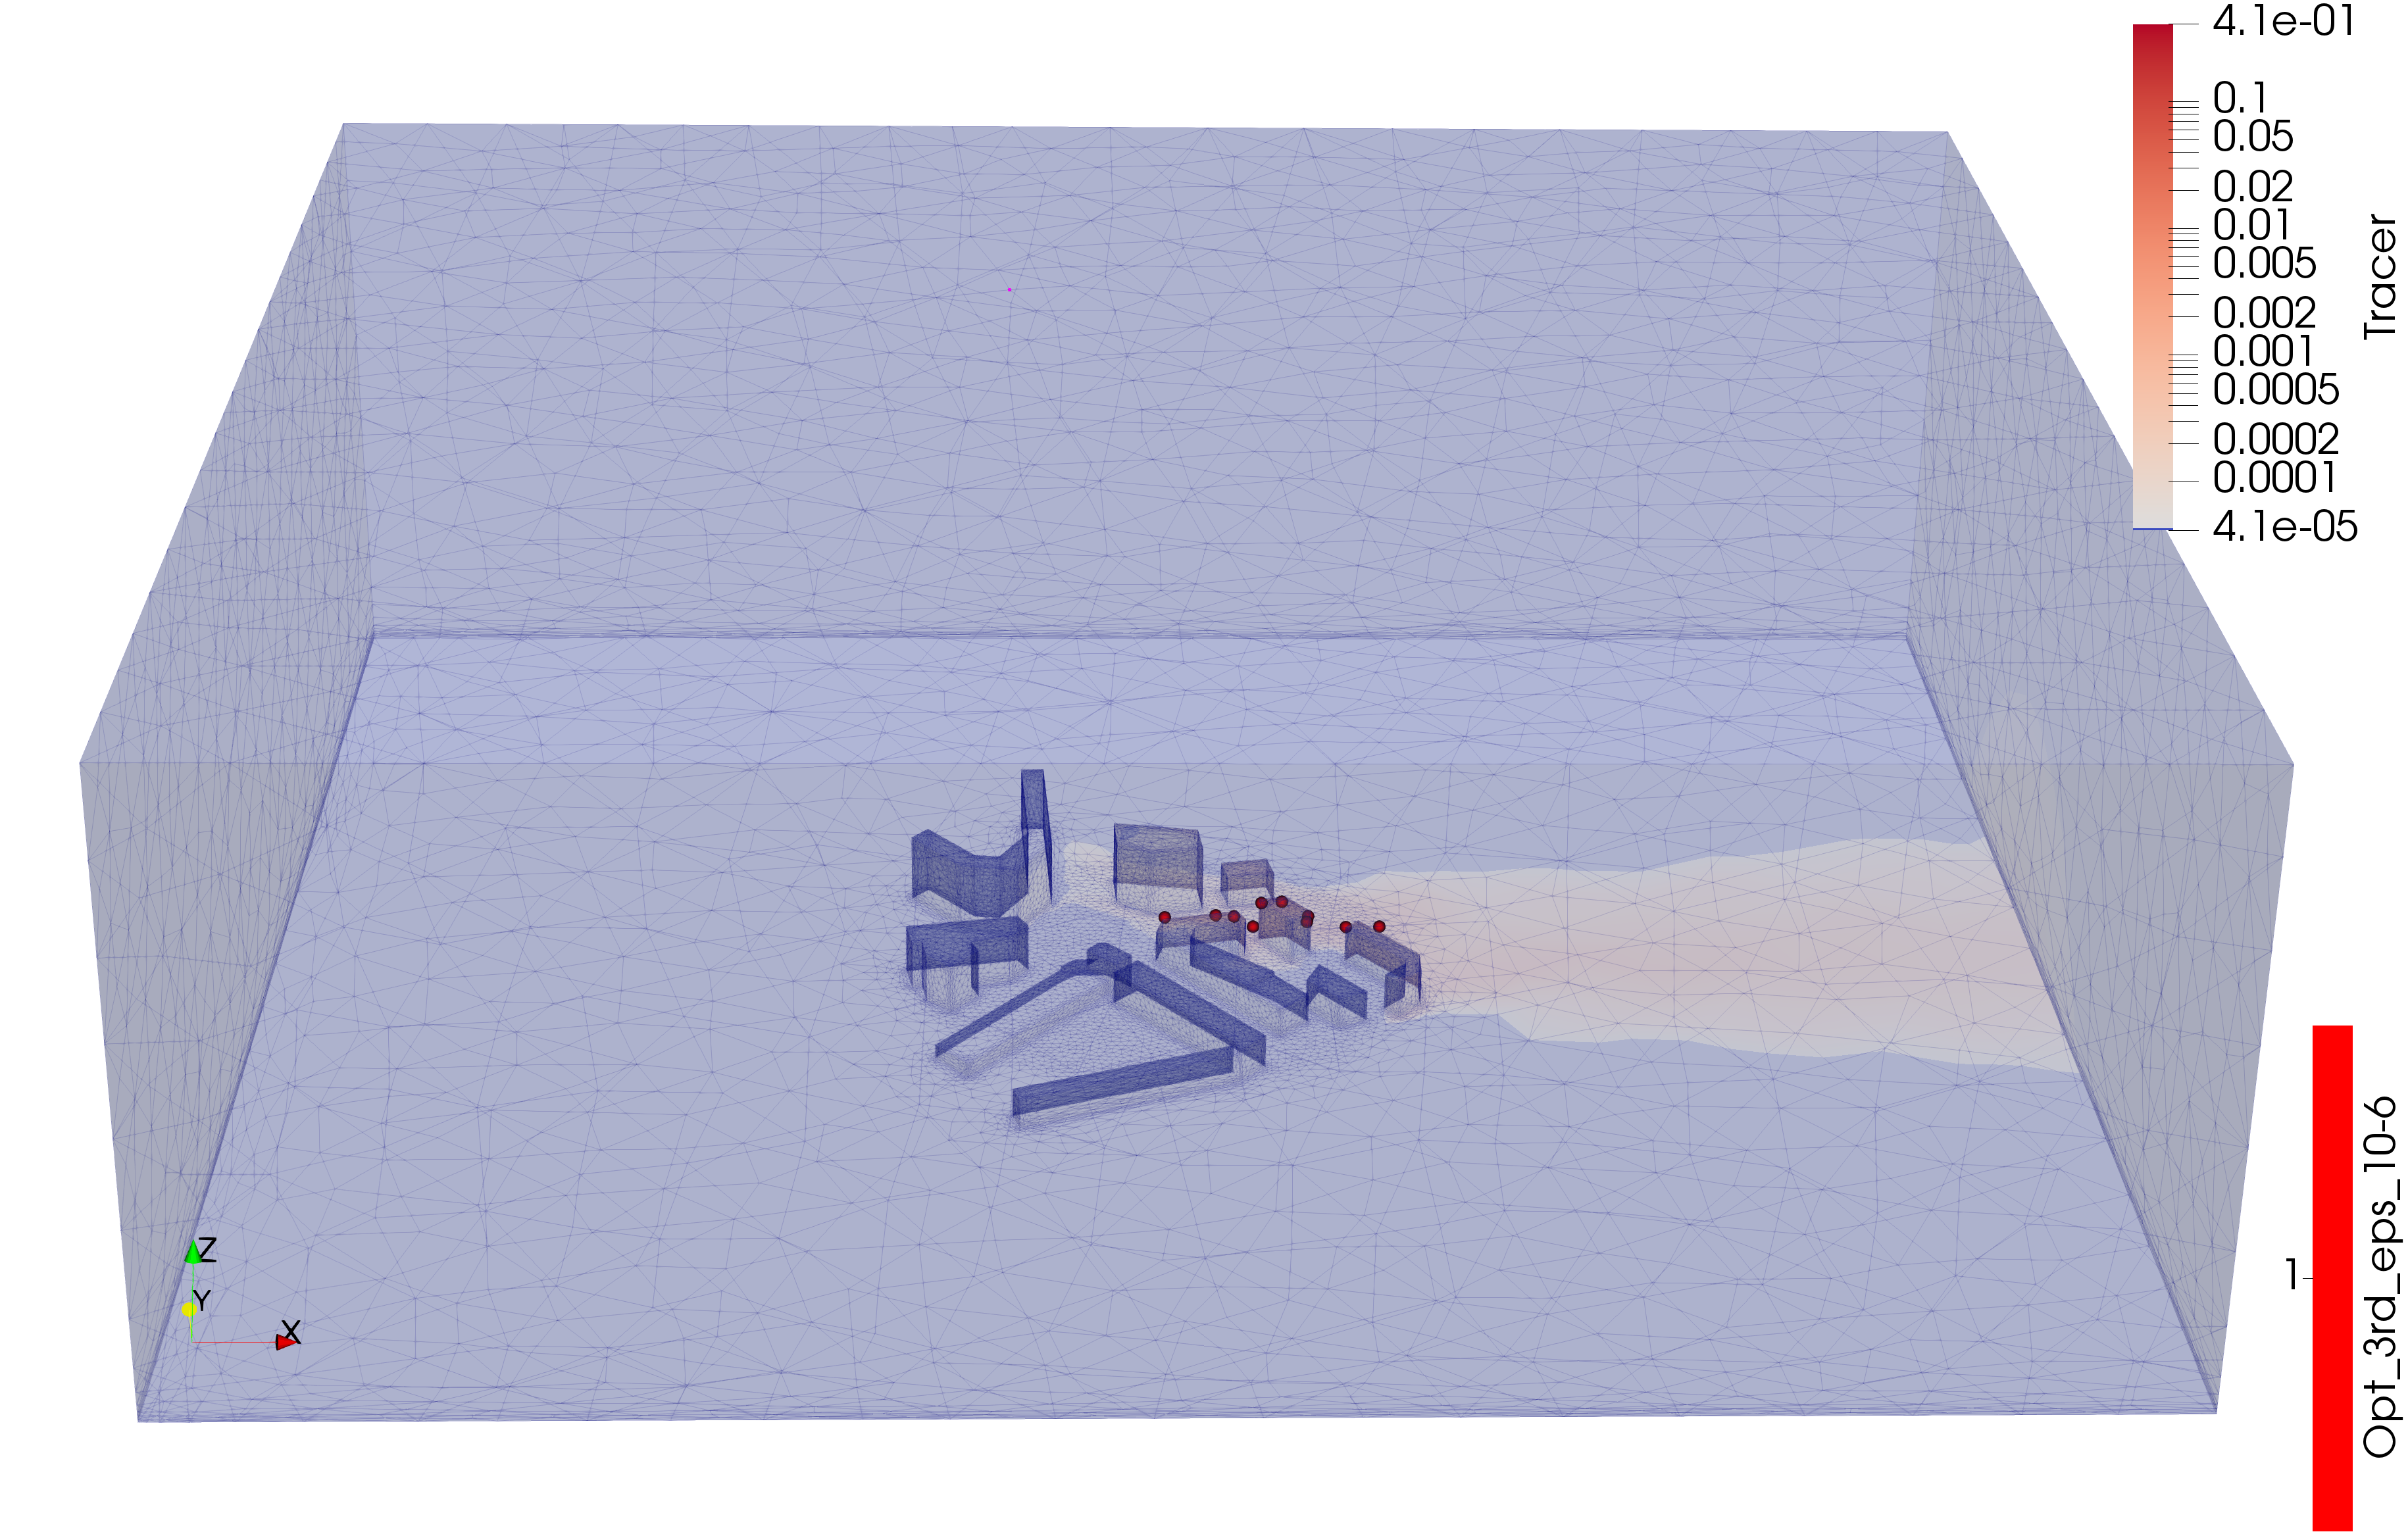
\includegraphics[width=0.7\linewidth]{figures/MainOptimResults/alg3opteps10-6_sideall_screenshot}
\smallbreak
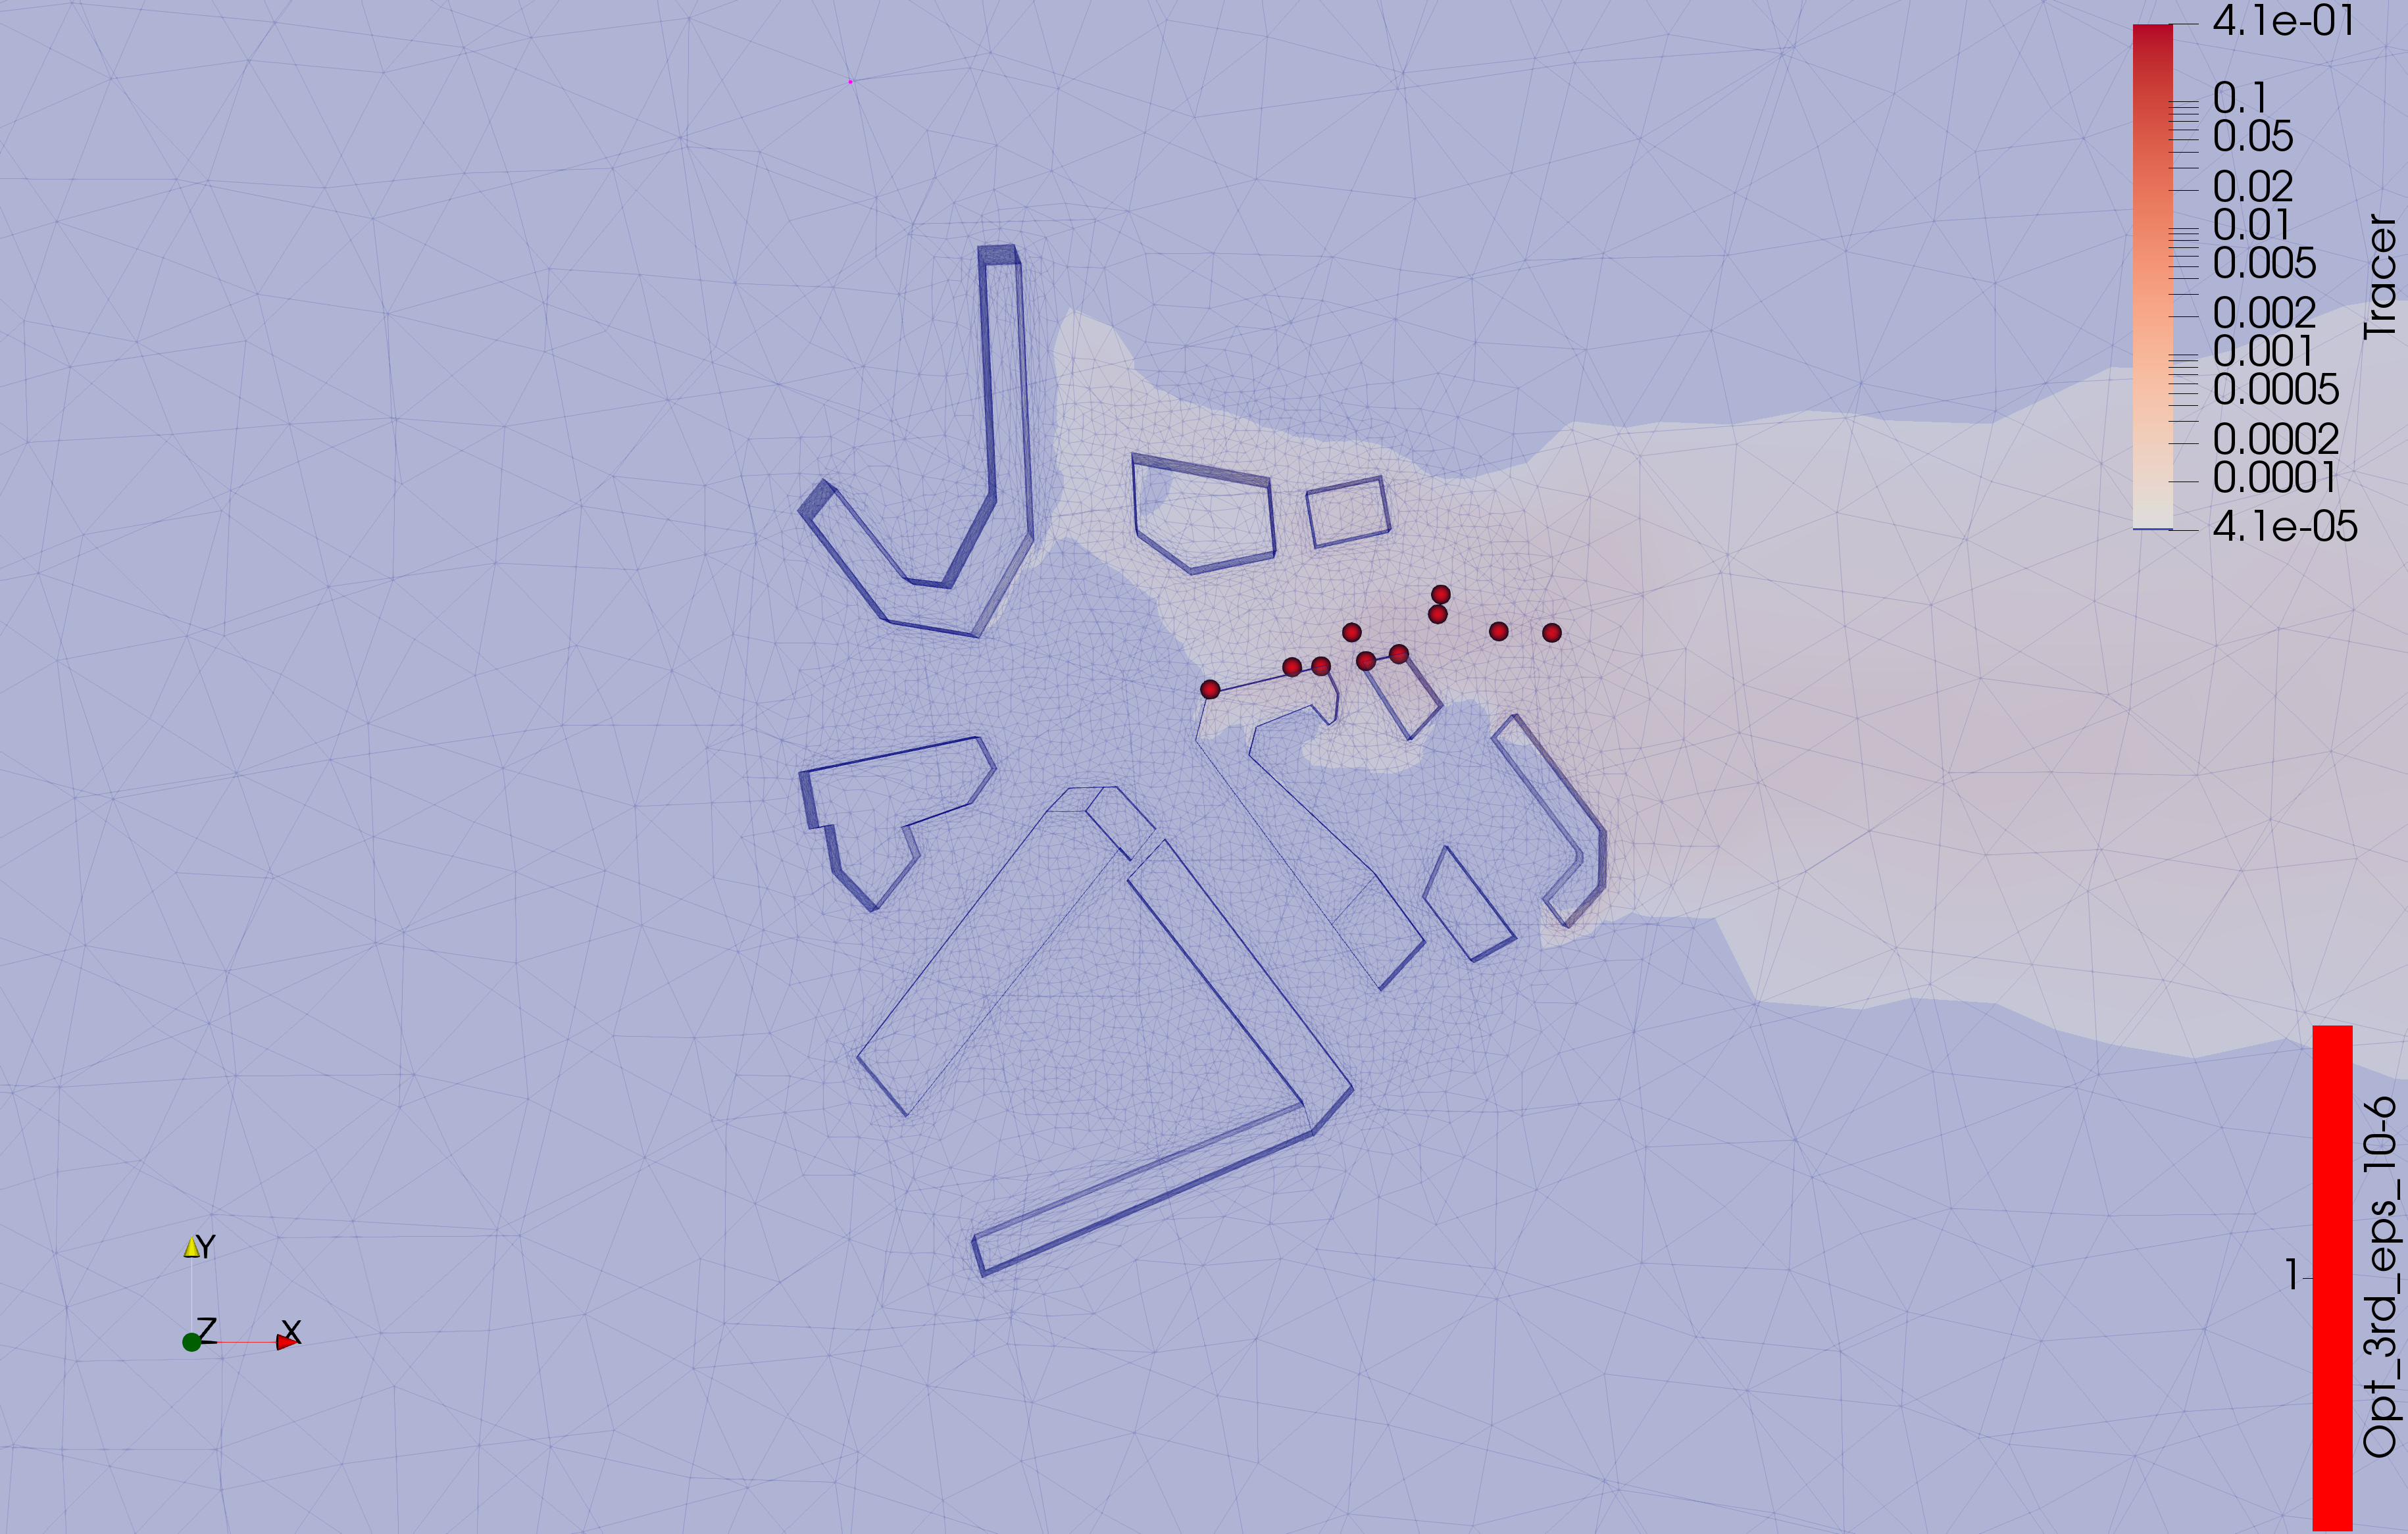
\includegraphics[width=0.7\linewidth]{figures/MainOptimResults/alg3opteps10-6_top_screenshot}
\smallbreak
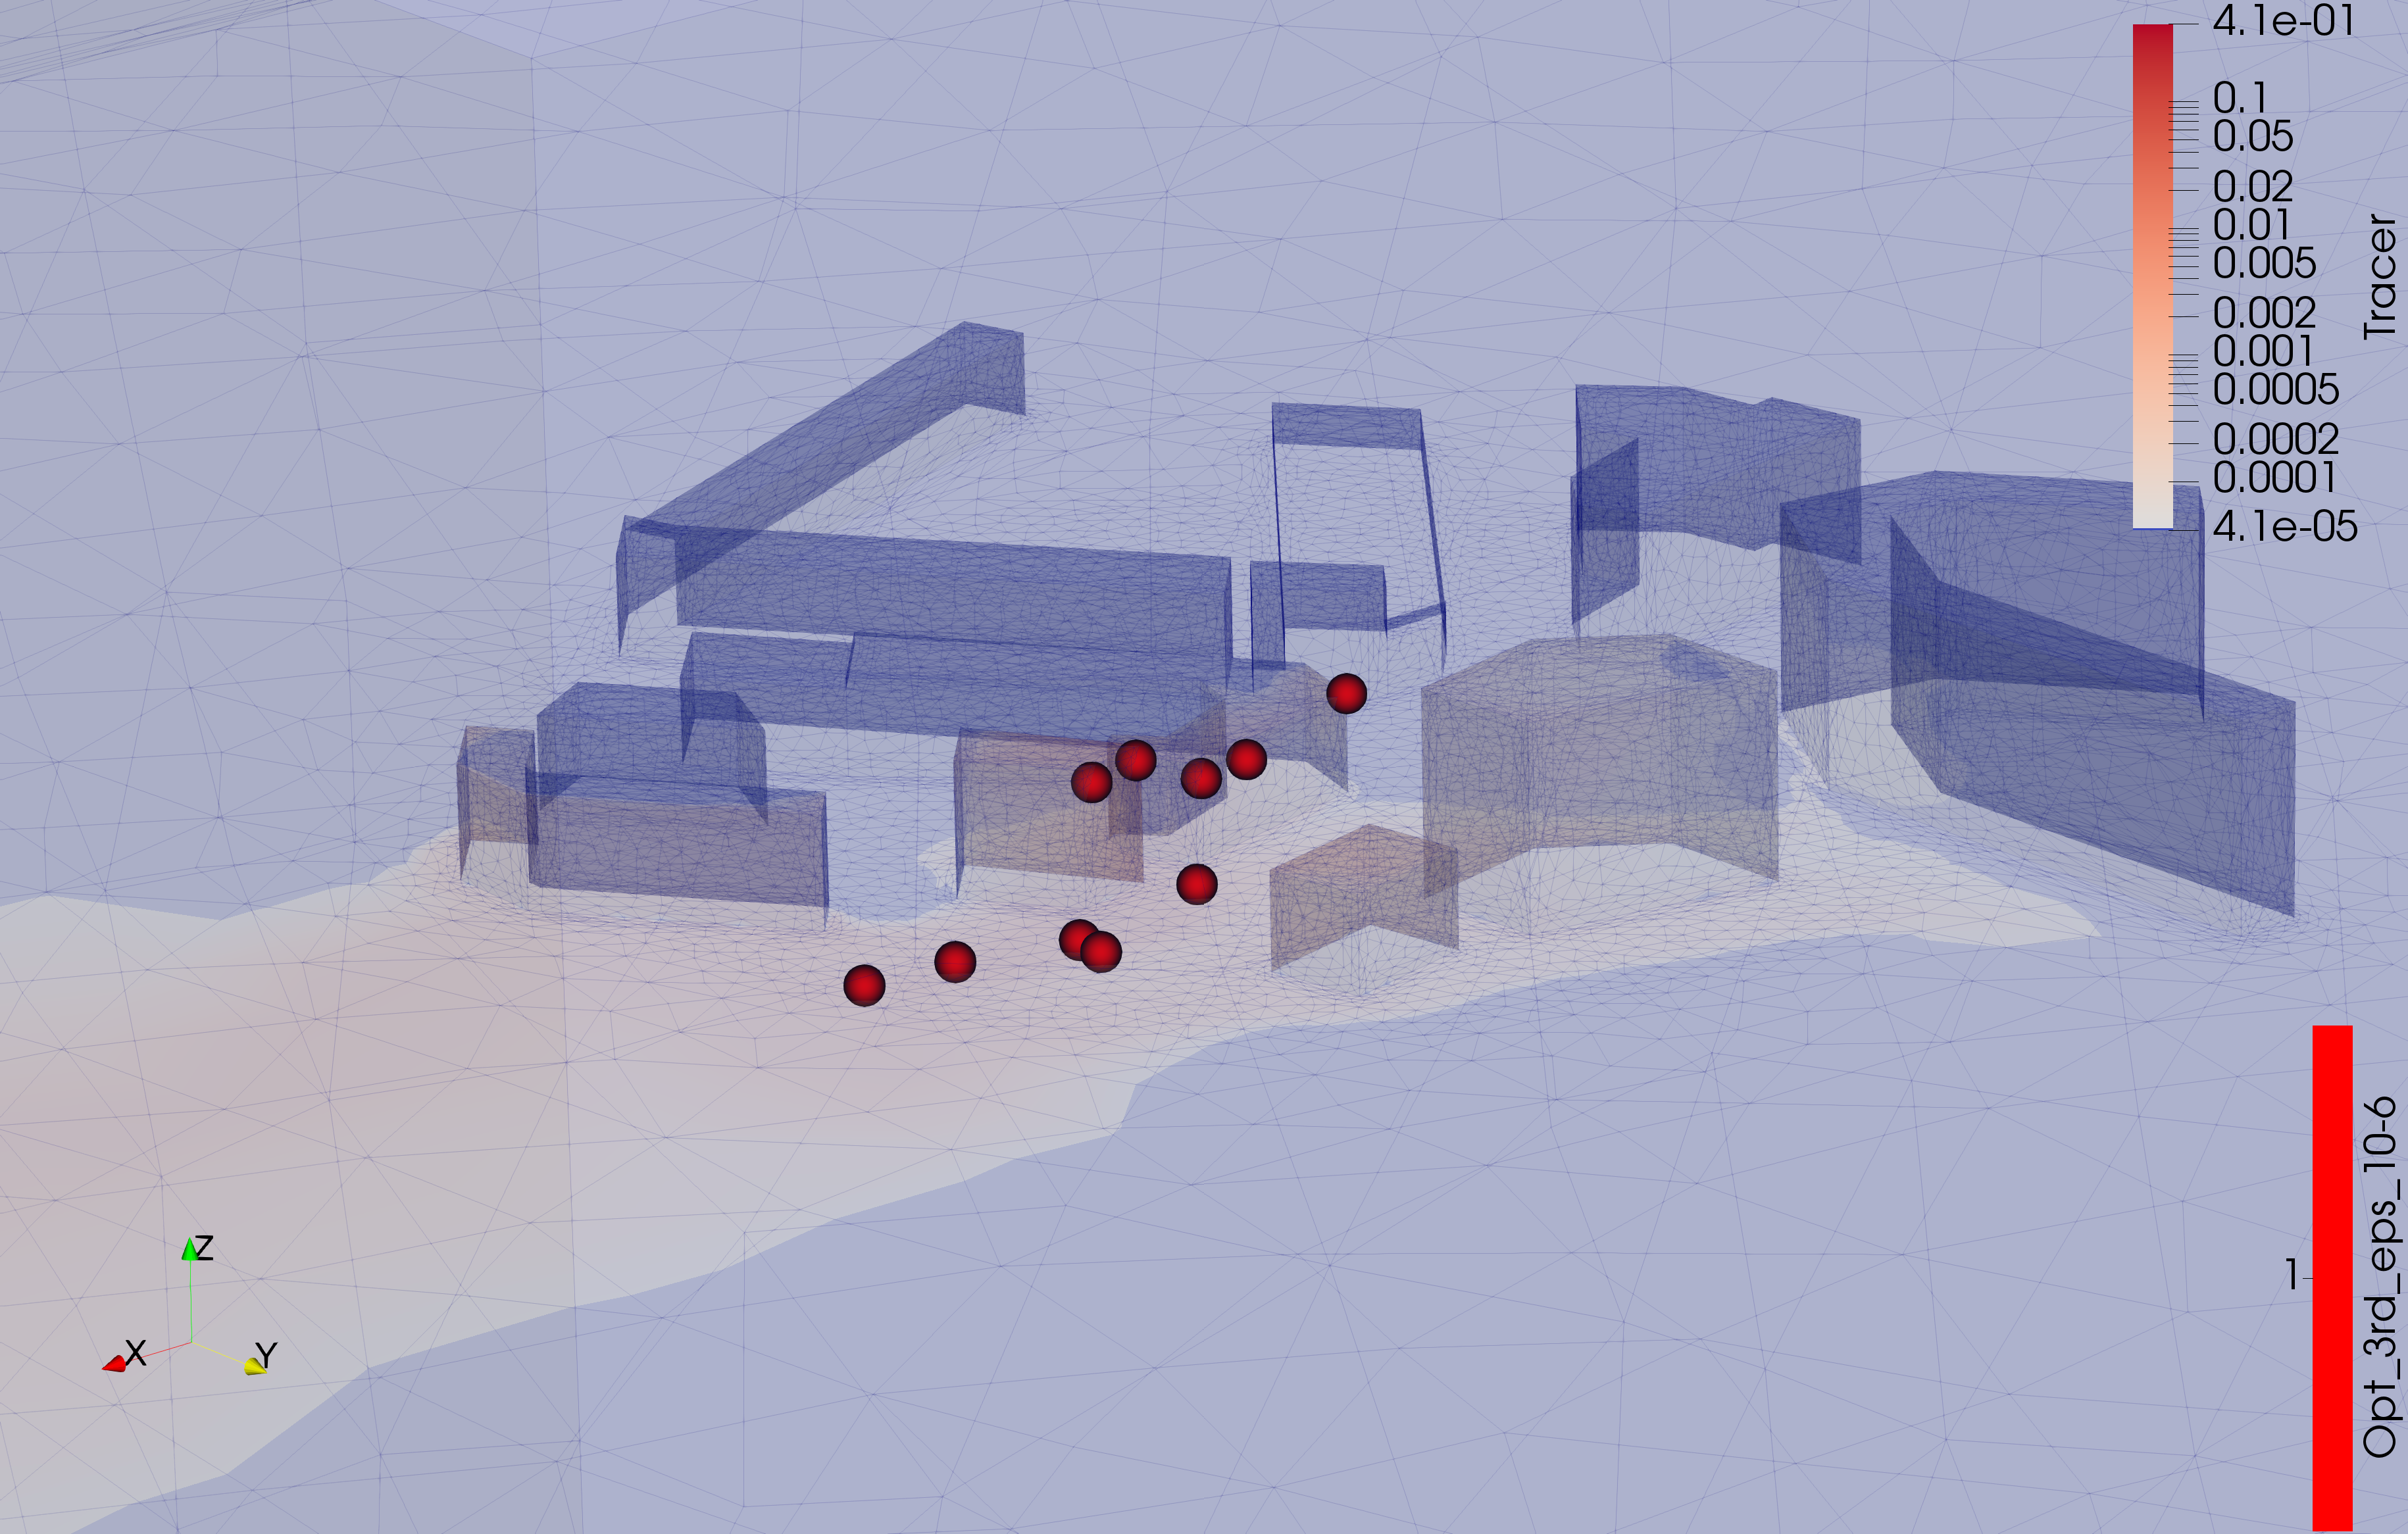
\includegraphics[width=0.7\linewidth]{figures/MainOptimResults/alg3opteps10-6_zoom_screenshot}
\caption{Position of the Optimal Set}
\label{fig:full_set:position:zoom}
\end{figure}


\paragraph{Description}

The location of our optimal set of points is split between points situated on the buildings (5 points) and around the ground level (5 points). They are situated in the middle of the tracer concentration beam and are close to the centre of the domain where the mesh density is maximal. \\ 

The points are roughly aligned in the wind direction, which is a good thing because the tracer is propagating itself from the centre of the domain, pushed by the wind in the east direction. Points along this direction are less correlated with each other than points perpendicular to this direction, as the tracer reaches them at the same time. Therefore it makes sense that the selected points are roughly along the wind direction as it will maximise the information retrieved during the propagation of the tracer. \\

Finally we observe the Mutual information gain $\delta_{y^*}$ for each placed sensor on Figure \ref{fig:full_set_Alg3:MIGAIN}. It confirms that our MI is sub-modular as here again the decreasing of the MI difference is monotonic. 
 \\


\begin{figure}[h]
\centering
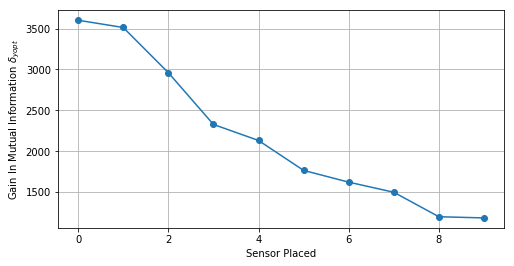
\includegraphics[width=0.6\linewidth]{figures/MainOptimResults/alg3opteps10-6_DeltaY}
\caption{Mutual Information Gain for each sensor - Algorithm 3}
\label{fig:full_set_Alg3:MIGAIN}
\end{figure}




\subsection{Lazy Algorithm with TSVD} \label{sec:res:TSVD}

We apply on the same dataset the 2nd Algorithm with the approximated GP that we defined earlier. We use the truncation parameter $\tau_{opt} = 25$. The results we obtain are displayed in table \ref{tab:tsvd:data} and Figure \ref{fig:full_set_tsvd:position:zoom}, along with the previous optimal results. \\ 
 
This algorithm computes the following results in $18083.87$ seconds or $5.02$ hours. 
 
 \paragraph{Description}

Here again, the location of our optimal set of points is split between points situated on the buildings (3 points) and around the ground level (7 points). The locations are more spread than the other set of points. Two locations are even at the border of the candidate dataset. The NN distance between this set and the previous one is $13.84$m,  which is not very important with regards to the size of the space.  \\ 




\begin{table}[h]
\centering
\footnotesize
\begin{tabular}{l|rrrrrrrrrr}
\toprule
$\A^*$ &  38726 &  14276 &  91348 &  5338  &  40994 &  29626 &  65851 &  65734 &  851   &  2293  \\
\midrule
X & -50.50 &  35.63 &  43.05 & 137.58 &  80.34 &  27.79 &  49.54 &  54.59 &  77.54 &  62.03 \\
Y &  48.85 &  58.69 &  27.51 &  55.78 &  76.20 &  26.24 &  28.88 &  25.42 &  34.82 &  41.92 \\
Z &  14.84 &   0.20 &   7.76 &   0.20 &   0.20 &  12.06 &  17.65 &   3.80 &   0.20 &   0.20 \\
\bottomrule
\end{tabular}
\caption{Optimal Points Locations TSVD - Tracer}
\label{tab:tsvd:data}
\end{table}


\begin{figure}[h!]
\centering
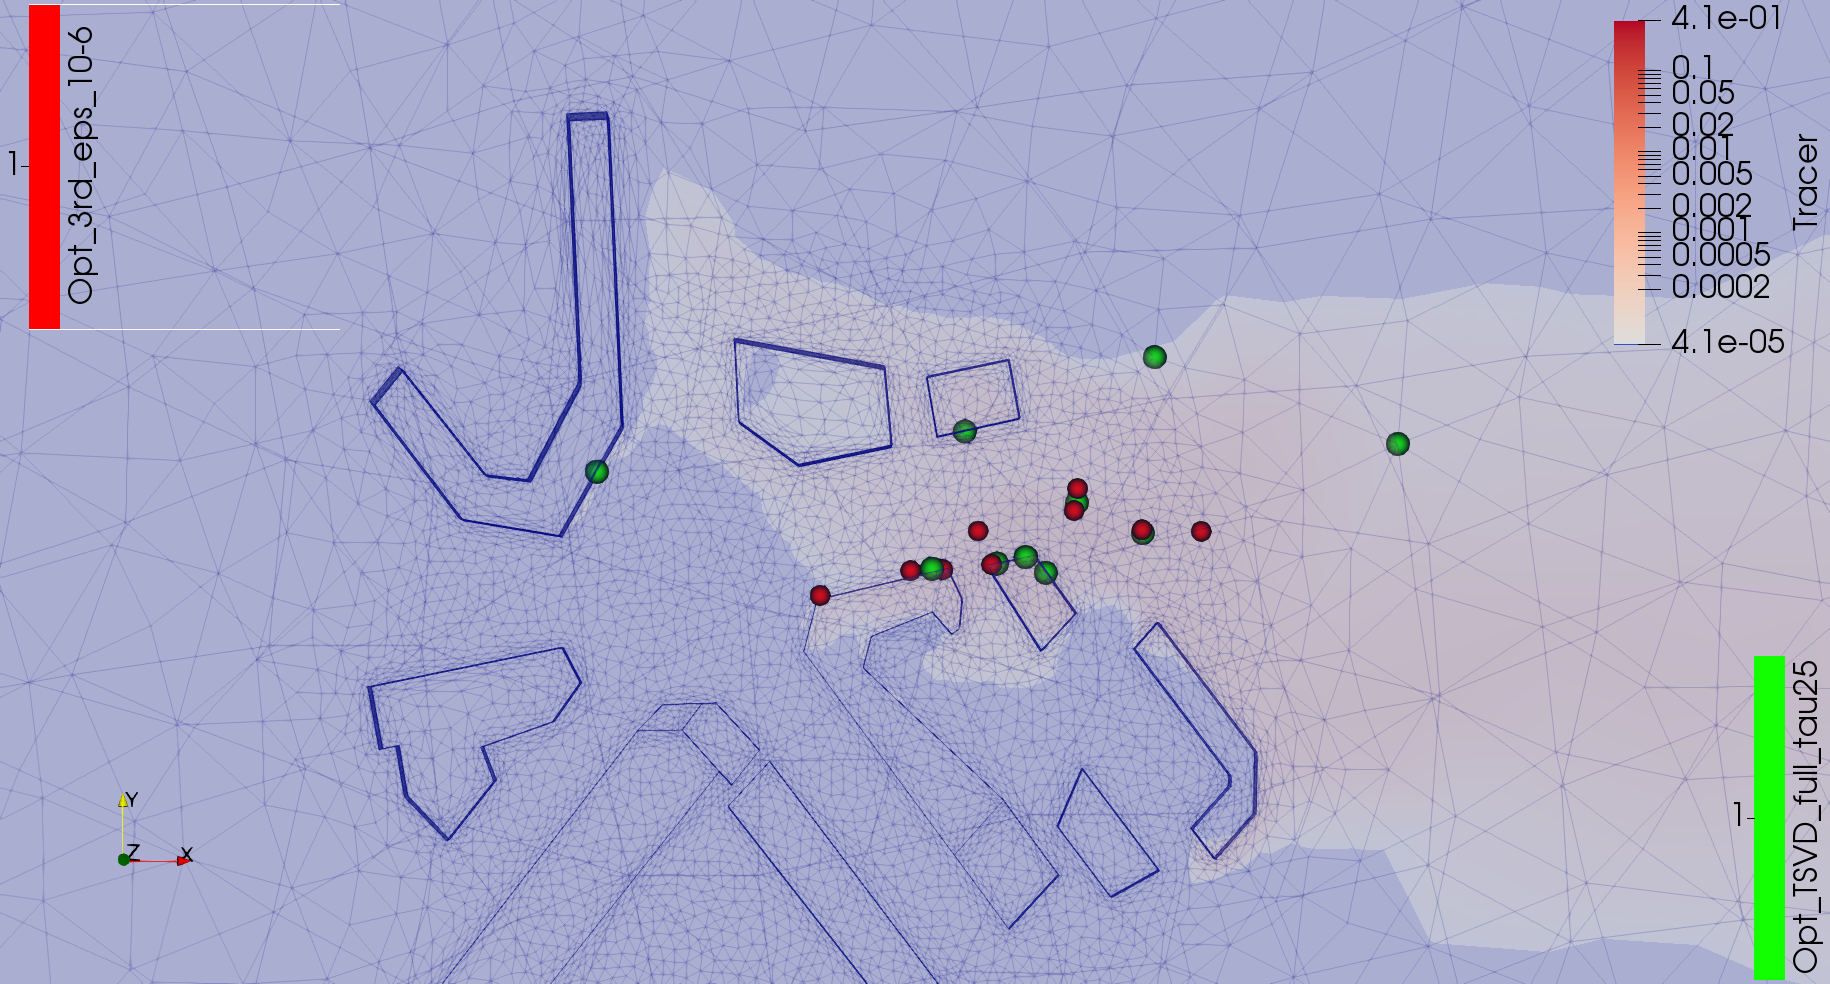
\includegraphics[width=0.7\linewidth]{figures/MainOptimTSVD/tsvd+3rd_position_top}
\smallbreak
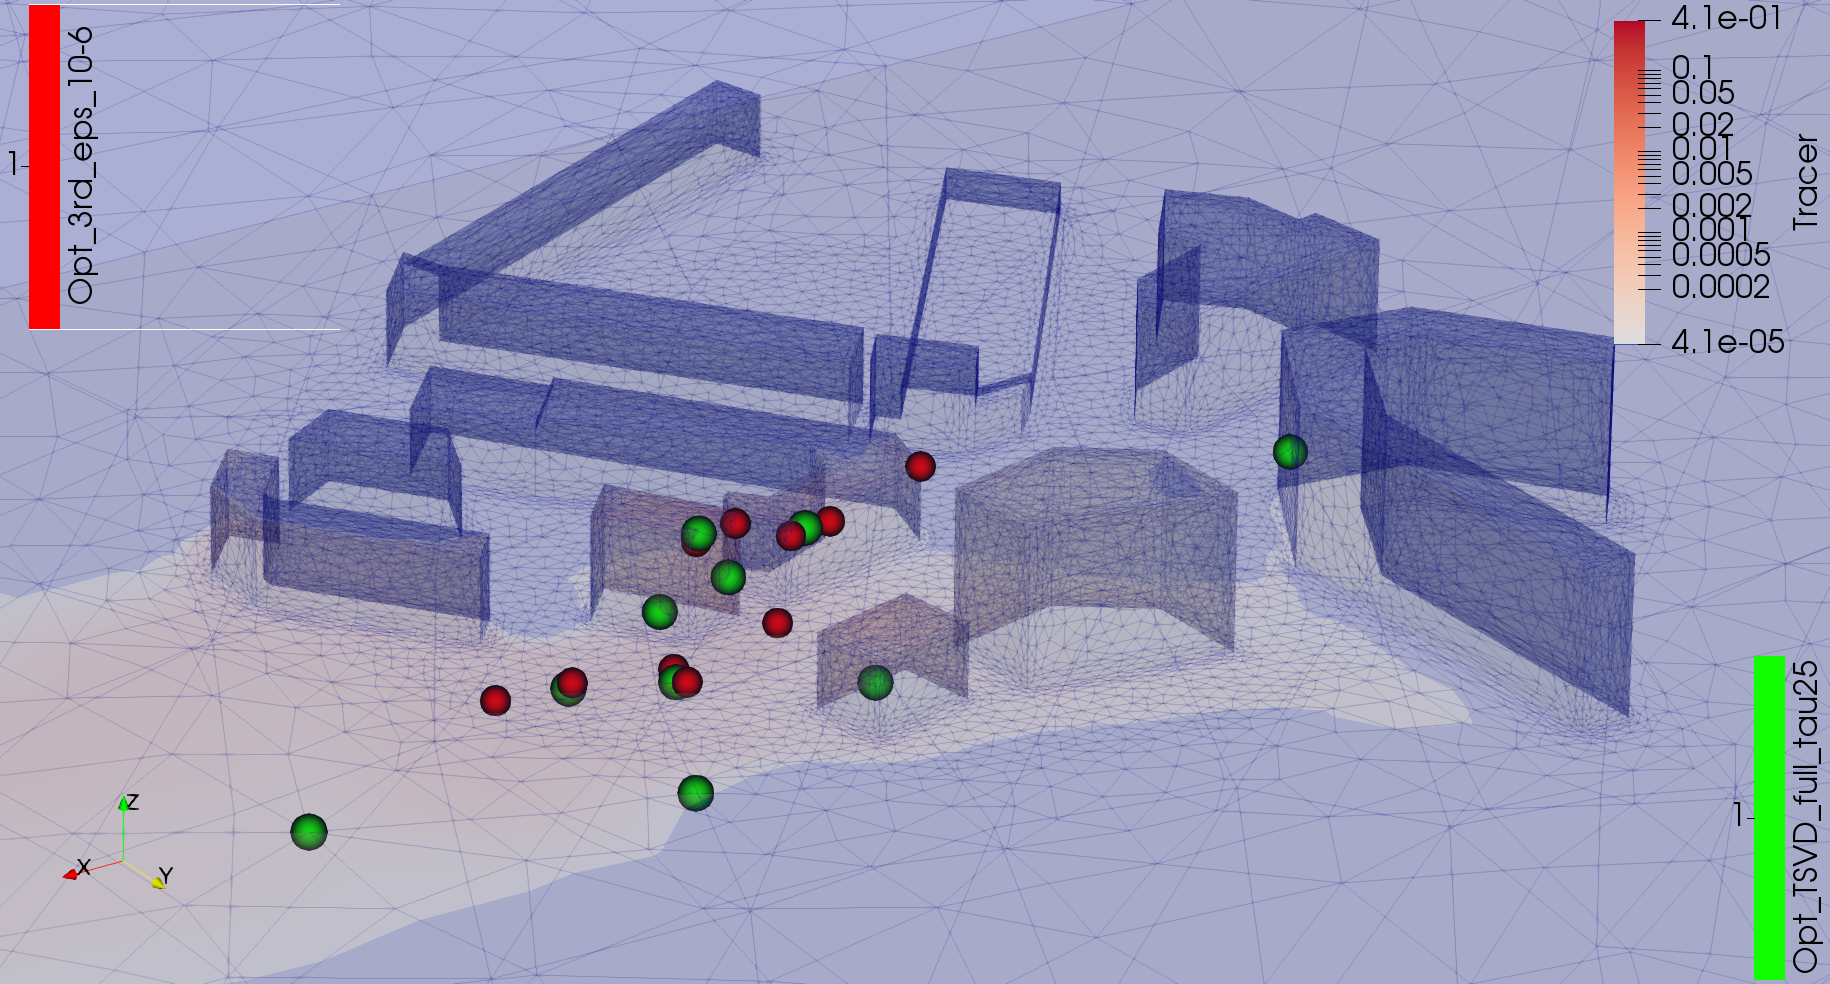
\includegraphics[width=0.7\linewidth]{figures/MainOptimTSVD/tsvd+3rd_position_side}
\caption{Position of the Optimal Set: Main View $\tau = 25$}
\label{fig:full_set_tsvd:position:zoom}
\end{figure}


Finally we observe the Mutual information gain $\delta_{y^*}$ for each placed sensor on Figure \ref{fig:full_set_tsvd:MIGAIN} is also constantly decreasing. However we can observe that it is not linear, as it was in the small set experimentation and in the Algorithm 3 optimisation. 
\\

\begin{figure}[h!]
\centering
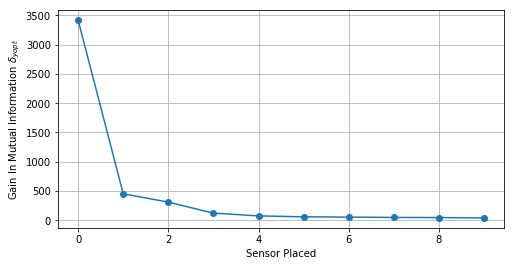
\includegraphics[width=0.6\linewidth]{figures/MainOptimTSVD/MIGain}
\caption{Mutual Information difference for each sensor - TSVD}
\label{fig:full_set_tsvd:MIGAIN}
\end{figure}




%
%\subsection{Optimisation on Pressure}
%
%
%
%\begin{table}[h]
%\centering
%\footnotesize
%    \begin{tabular}{l|rrrrrrrrrr}
%\toprule
%$\A^*$ &  72496 &  75832 &  85761 &  86497 &  26107 &  17851 &  36552 &  38178 &  3351  &  36551 \\
%\midrule
%X & -54.41 & -46.24 & -51.00 & -42.50 & -52.34 & -50.68 & -49.55 & -48.37 & -52.88 & -54.55 \\
%Y &  70.39 &  95.22 &  72.66 & 132.29 &  31.07 &  31.96 &  32.72 &  33.31 &  28.94 &  26.82 \\
%Z &   8.70 &   3.28 &  29.14 &   1.37 &   1.16 &   0.20 &   1.44 &   0.80 &   0.20 &   0.20 \\
%\bottomrule
%\end{tabular}
%\caption{\caption{Optimal Points Locations - Pressure}
%\end{table}
%
%\todo{Fill Pressure Data Optimisation}



%%%%%%%%% OPTIMISATION %%%%%%%%

\section{Application to Variational DA}


As we have seen, one way of applying the results to a real situation is to proceed to a Variational Data Assimilation of the points selected. By taking results of a simulation and applying DA on our selected points we can try to see if the results are usable in the context of the MAGIC project. 

\subsection{Parameters of the Experiment} 

For this experiment, we chose to consider the same simulation data than previously: the 3D smallLSBU.  We choose as the observation state, the step $988$ of the simulation, and as background state, the step $100$ of the simulation. \\

We compute the Variational DA on the 10 optimal points selected by the algorithms and compute the background error and the error after the DA procedure.  
%\subsection{VarDA on Tracer Concentration}
%
%First we apply our DA algorithm on the \textit{Tracer} Data. 

\subsection{VarDA on Local Kernel Results}

First, we run the VarDa Algorithm and obtain the following. 
\begin{table}[h]
\centering
    \begin{tabular}{c|c|c}
    \toprule
          MSE [xDA] & MSE [xB] &  Imp. [xDA / xB] \\ \midrule
         $7.7375 \cdot 10^{-17}$ &  $0.9923$ & $7.7975 \cdot 10^{-17}$ \\ \bottomrule
    \end{tabular}
    \caption{VarDA on Local Kernel Results. }
\end{table}

\paragraph{Comparison to Random}

To compare those results to another set of points, we proceed as follows. Around every single point of $\A^*$, we select randomly (uniformly) a point located within a radius of $R=10m$. This allows us to compare the results to some random set that is close to the optimum. We then proceed to $1'000$ different random selection and compute the average errors and their standard deviations, stated in table \ref{tab:varDa:random}. \\


\begin{table}[h]
\centering
\begin{tabular}{l|cc}
\toprule
               & Average & Std Dev \\ \midrule
MSE [xDA]      & $6.1008 \cdot 10^{-17}$  & $4.1680 \cdot 10^{-17}$  \\
MSE [xB]       & $0.6538$  & $0.1718$  \\
Imp. Ratio [xDA / xB]  &   $9.3313 \cdot 10^{-17}$  & - \\ \bottomrule
\end{tabular}
    \caption{VarDA on $1'000$ Near Random Points: Local Kernel Results}
    \label{tab:varDa:random}
\end{table}

\paragraph{Analysis}

We can see that the error of the optimal set $\A^*$ is very small on the DA results, almost negligible. The improvement form the pre-assimilation background error is of almost $100\%$. This shows that this set of points has some good properties for Data Assimilation. \\

By comparing those results to the $1'000$ random samples, we see that the average is very close to the error of the optimal set. However, the improvement from the background error is smaller for the random sets. In this way, we have better results for the optimal set of points.  



\subsection{VarDA on Gaussian Approximation Results}

We then run the same algorithm on the optimal set found with the lazy algorithm combined with TSVD GP approximation. 

\begin{table}[h]
\centering
    \begin{tabular}{c|c|c}
    \toprule
          MSE [xDA] & MSE [xB] &  Imp. Ratio [xDA / xB] \\ \midrule
        $9.8945 \cdot 10^{-17}$  &  $1.1354$ & $8.7145 \cdot 10^{-17} $ \\ \bottomrule
    \end{tabular}
    \caption{VarDA on TSVD Results. }
\end{table}

\paragraph{Comparison to Random}

To compare those results to another set of points we proceed as previously. The results for $1'000$ random sets sampled at a $10$m radius from each optimal points are given in table \ref{tab:TSVD:random}. 
 \\


\begin{table}[h]
\centering
\begin{tabular}{l|cc}
\toprule
               & Average & Std Dev \\ \midrule
MSE [xDA]       & $6.6843 \cdot 10^{-17}$  & $4.9458 \cdot 10^{-17}$  \\
MSE [xB]  & $0.6725$  & $0.2148$  \\
Improvement Ratio  [xDA / xB]  & $9.9381 \cdot 10^{-17}$  & - \\ \bottomrule
\end{tabular}
    \caption{VarDA on 500 Random Points: TSVD Results}
    \label{tab:TSVD:random}
\end{table}

\paragraph{Analysis}

We observe the same phenomenon than with the \textit{Tracer} Local Kernel results. The DA error is negligible and the Improvement is better with our optimal points. 


%\subsection{VarDA on Pressure}
%
%Now we apply the DA procedure to the \textit{Pressure} Data. 
%
%\subsubsection{VarDA on Local Kernel Results}
%
%\subsubsection{VarDA on Gaussian Approximation Results}
%




\subsection{Limitations of the Application}

Even if the error magnitude is not decreasing, we can see an improvement in the value of the computed ratio between the DA error and the background error. It has been shown by \citet{arcucci_optimal_2019}, that when the simulation is continued after DA, the an initial improvement is propagated and an initial better improvement leads to better results overall for both the sensors and un-monitored spaces. 

%As we have seen the results given by this simple VarDA application are not very satisfying. We observe clearly that the randomly selected points give results \textbf{as good as} the optimal points. \\

We are here measuring the error directly after the assimilation and only on the 10 assimilated points. As VarDA is an optimisation problem that minimises this error,  considering the small number of points and the fact that there is no dimensionality reduction of the deviation matrix, it is quite natural that this error is negligible.  \\

To draw more conclusions on the validity of our set of points, we would need to continue the simulation after the DA procedure and compare after some time the states of all the points of the space with different assimilated sets of points. \\



% Furthermore, we have to consider the DA as a simple application of our near-optimal sensor positioning algorithm. We have not proven any link between the Mutual Information criterion, that we had optimised to find the optimal points, and the optimality of the DA procedure. \\
 
% Not taking into account the dynamics of the space. Assumption of samples are independent and identically distributed and samples of the sample Gaussian probability distribution. 

% We have to keep in mind the DA Algorithm used is computing the MSE only on the 10 points of interest. We do not study here the propagation after the DA, so we are not able to see the impact of our selected set on the rest of the locations of the space. \\


